\batchmode
\documentclass[a4paper]{book}
\usepackage{makeidx}
\usepackage{natbib}
\usepackage{graphicx}
\usepackage{multicol}
\usepackage{float}
\usepackage{listings}
\usepackage{color}
\usepackage{ifthen}
\usepackage[table]{xcolor}
\usepackage{textcomp}
\usepackage{alltt}
\usepackage[utf8]{inputenc}
\usepackage{mathptmx}
\usepackage[scaled=.90]{helvet}
\usepackage{courier}
\usepackage{sectsty}
\usepackage[titles]{tocloft}
\usepackage{doxygen}
\lstset{language=C++,inputencoding=utf8,basicstyle=\footnotesize,breaklines=true,breakatwhitespace=true,tabsize=8,numbers=left }
\makeindex
\setcounter{tocdepth}{3}
\renewcommand{\footrulewidth}{0.4pt}
\renewcommand{\familydefault}{\sfdefault}
\hfuzz=15pt
\setlength{\emergencystretch}{15pt}
\hbadness=750
\tolerance=750
\begin{document}
\begin{titlepage}
\vspace*{7cm}
\begin{center}
{\Large dish\-\_\-viz }\\
\vspace*{1cm}
{\large \-Generated by Doxygen 1.7.6.1}\\
\vspace*{0.5cm}
{\small Wed Feb 6 2013 18:34:42}\\
\end{center}
\end{titlepage}
\clearemptydoublepage
\pagenumbering{roman}
\tableofcontents
\clearemptydoublepage
\pagenumbering{arabic}
\chapter{\-Main \-Page}
\label{index}

{\bfseries arm} is a \-R\-O\-S package for controlling a \-Manus \-A\-R\-M. \-The package consists of one control node and two teleop nodes. \-You must have a \-Manus \-A\-R\-M properly connected and configured in order for this package to be of any use. \-You must have both a teleop node and the control node running in order to move the \-A\-R\-M. \-There is a node for keyboard teleop and a node for neuron dish activity teleop.\section{\-Code A\-P\-I}\label{index_codeapi}

\begin{DoxyItemize}
\item \-Start the \-A\-R\-M control node by creating an \doxyref{\-Arm\-Control}{p.}{classArmControl} object.
\item \-Start the dish teleop node by creating a \doxyref{\-Teleop\-Arm\-Dish}{p.}{classTeleopArmDish} object.
\item \-Start the keyboard teleop node by creating a \doxyref{\-Teleop\-Arm\-Key}{p.}{classTeleopArmKey} object.
\end{DoxyItemize}


\begin{DoxyItemize}
\item \-To get an instance of the \-A\-R\-M\-: \doxyref{\-Manus\-Arm\-::instance}{p.}{classManusArm_a70516aaf8fa75276f7bb7bcd1912671c}
\item \-To init the \-A\-R\-M\-: \doxyref{\-Manus\-Arm\-::init}{p.}{classManusArm_aeb2e212f64c683e45a6f5bb90afb1a70}
\item \-To move the \-A\-R\-M\-: \doxyref{\-Manus\-Arm\-::move\-Cartesian}{p.}{classManusArm_a66cd2a077fbcdc00d19c76677c900380} and \doxyref{\-Manus\-Arm\-::move\-Constant}{p.}{classManusArm_ab76c4573bfc84e4ce5fe2ad36a8b2522}
\item \-To check if cartesian movement is finished\-: \doxyref{\-Manus\-Arm\-::is\-Move\-Complete}{p.}{classManusArm_a1cff3017b09dfaace5f2c9ca4844d21e}
\item \-To end cartesian movement early\-: \doxyref{\-Manus\-Arm\-::set\-Move\-Complete}{p.}{classManusArm_a4369585e90bd37e57dab71c0e7771d8a}
\item \-To fold/unfold\-: \doxyref{\-Manus\-Arm\-::fold}{p.}{classManusArm_a379092d8f07c767962911d2a410d9d63} and \doxyref{\-Manus\-Arm\-::unfold}{p.}{classManusArm_a29b633fe436ba500058634b8e0a029e5}
\item \-To get joint positions\-: \doxyref{\-Manus\-Arm\-::get\-Print\-State}{p.}{classManusArm_ac6fa919efbacf860202362c1b3611f48} and \doxyref{\-Manus\-Arm\-::get\-Csv\-State}{p.}{classManusArm_a7584b3f88ddc538a8308d7bb7ff1fb89}
\end{DoxyItemize}\section{\-R\-O\-S A\-P\-I}\label{index_rosapi}
\-List of nodes\-:
\begin{DoxyItemize}
\item {\bfseries arm\-\_\-control} 
\item {\bfseries teleop\-\_\-arm\-\_\-dish} 
\item {\bfseries teleop\-\_\-arm\-\_\-key} 
\end{DoxyItemize}



\subsection{arm\-\_\-control}\label{index_arm_control}
arm\-\_\-control controls the \-A\-R\-M. \-It receives movement commands from teleop nodes and moves the arm hardware appropriately.\subsubsection{\-Usage}\label{index_Usage}
\begin{DoxyVerb}
$ rosrun arm arm_control
\end{DoxyVerb}
\subsubsection{\-R\-O\-S topics}\label{index_topics}
\-Subscribes to\-:
\begin{DoxyItemize}
\item {\bfseries \char`\"{}cartesian\-\_\-moves\char`\"{}}\-: [arm/cartesian\-\_\-moves] cartesian movement commands
\item {\bfseries \char`\"{}constant\-\_\-moves\char`\"{}}\-: [arm/constant\-\_\-move] constant movement commands
\item {\bfseries \char`\"{}constant\-\_\-move\-\_\-times\char`\"{}}\-: [arm/constant\-\_\-move\-\_\-time] constant movement by time commands
\end{DoxyItemize}

\-Publishes to\-:
\begin{DoxyItemize}
\item {\bfseries \-N/\-A} 
\end{DoxyItemize}\subsubsection{\-R\-O\-S parameters}\label{index_parameters}
\-Reads the following parameters from the parameter server


\begin{DoxyItemize}
\item {\bfseries \-N/\-A} 
\end{DoxyItemize}

\-Sets the following parameters on the parameter server


\begin{DoxyItemize}
\item {\bfseries \-N/\-A} 
\end{DoxyItemize}\subsubsection{\-R\-O\-S services}\label{index_services}

\begin{DoxyItemize}
\item {\bfseries \char`\"{}time\-\_\-service\char`\"{}}\-: [time\-\_\-server/time\-\_\-srv] polls system time to keep the node in sync
\end{DoxyItemize}



\subsection{teleop\-\_\-arm\-\_\-dish}\label{index_teleop_arm_dish}
teleop\-\_\-arm\-\_\-dish creates movement commands for the arm based on \-C\-A\-T (center of activity trajectory) data received from the \-C\-A\-T creator node.\subsubsection{\-Usage}\label{index_Usage}
\begin{DoxyVerb}
$ rosrun arm teleop_arm_dish
\end{DoxyVerb}
\subsubsection{\-R\-O\-S topics}\label{index_topics}
\-Subscribes to\-:
\begin{DoxyItemize}
\item {\bfseries \char`\"{}cats\char`\"{}}\-: [burst\-\_\-calc/cat] center of activity trajectories
\end{DoxyItemize}

\-Publishes to\-:
\begin{DoxyItemize}
\item {\bfseries \char`\"{}cartesian\-\_\-moves\char`\"{}}\-: [arm/cartesian\-\_\-moves] cartesian movement commands
\item {\bfseries \char`\"{}constant\-\_\-move\-\_\-times\char`\"{}}\-: [arm/constant\-\_\-move\-\_\-time] constant movement by time commands
\end{DoxyItemize}\subsubsection{\-R\-O\-S parameters}\label{index_parameters}
\-Reads the following parameters from the parameter server


\begin{DoxyItemize}
\item {\bfseries arm\-\_\-speed} 
\item {\bfseries arm\-\_\-safe\-\_\-range} 
\item {\bfseries max\-\_\-range\-\_\-from\-\_\-midpoint} 
\end{DoxyItemize}

\-Sets the following parameters on the parameter server


\begin{DoxyItemize}
\item {\bfseries \-N/\-A} 
\end{DoxyItemize}\subsubsection{\-R\-O\-S services}\label{index_services}

\begin{DoxyItemize}
\item {\bfseries \char`\"{}time\-\_\-service\char`\"{}}\-: [time\-\_\-server/time\-\_\-srv] polls system time to keep the node in sync
\end{DoxyItemize}



\subsection{teleop\-\_\-arm\-\_\-key}\label{index_teleop_arm_key}
teleop\-\_\-arm\-\_\-key creates movement commands for the arm based on keyboard input.\subsubsection{\-Usage}\label{index_Usage}
\begin{DoxyVerb}
$ rosrun arm teleop_arm_key
\end{DoxyVerb}
\subsubsection{\-R\-O\-S topics}\label{index_topics}
\-Subscribes to\-:
\begin{DoxyItemize}
\item {\bfseries \-N/\-A} 
\end{DoxyItemize}

\-Publishes to\-:
\begin{DoxyItemize}
\item {\bfseries \char`\"{}constant\-\_\-moves\char`\"{}}\-: [arm/constant\-\_\-move] constant movement commands
\end{DoxyItemize}\subsubsection{\-R\-O\-S parameters}\label{index_parameters}
\-Reads the following parameters from the parameter server


\begin{DoxyItemize}
\item {\bfseries \-N/\-A} 
\end{DoxyItemize}

\-Sets the following parameters on the parameter server


\begin{DoxyItemize}
\item {\bfseries \-N/\-A} 
\end{DoxyItemize}\subsubsection{\-R\-O\-S services}\label{index_services}

\begin{DoxyItemize}
\item {\bfseries \-N/\-A} 
\end{DoxyItemize}\section{\-Command-\/line tools}\label{index_commandline}
\-There are several launch files available to simplify running all of the nodes. \-Each launch file has a corresponding parameter file. \-They are as follows\-:


\begin{DoxyItemize}
\item brian\-\_\-csv.\-launch
\item brian\-\_\-sim.\-launch
\item csv.\-launch
\item volt\-\_\-only\-\_\-brian\-\_\-csv.\-launch
\item volt\-\_\-only\-\_\-brian\-\_\-sim.\-launch
\item volt\-\_\-only\-\_\-csv.\-launch
\end{DoxyItemize}\subsection{\-Usage}\label{index_Usage}
\begin{DoxyVerb}
$ roslaunch [package] [file]
\end{DoxyVerb}


\begin{DoxyParagraph}{\-Example}

\end{DoxyParagraph}
\begin{DoxyVerb}
$ roslaunch arm csv.launch
\end{DoxyVerb}
 
\chapter{\-Namespace \-Index}
\section{\-Namespace \-List}
\-Here is a list of all namespaces with brief descriptions\-:\begin{DoxyCompactList}
\item\contentsline{section}{{\bf burst\-\_\-calc} }{\pageref{namespaceburst__calc}}{}
\item\contentsline{section}{{\bf burst\-\_\-calc\-::msg} }{\pageref{namespaceburst__calc_1_1msg}}{}
\item\contentsline{section}{{\bf burst\-\_\-calc\-::msg\-::\-\_\-burst} }{\pageref{namespaceburst__calc_1_1msg_1_1__burst}}{}
\item\contentsline{section}{{\bf burst\-\_\-calc\-::msg\-::\-\_\-ca} }{\pageref{namespaceburst__calc_1_1msg_1_1__ca}}{}
\item\contentsline{section}{{\bf burst\-\_\-calc\-::msg\-::\-\_\-cat} }{\pageref{namespaceburst__calc_1_1msg_1_1__cat}}{}
\item\contentsline{section}{{\bf burst\-\_\-calc\-::msg\-::\-\_\-ranges} }{\pageref{namespaceburst__calc_1_1msg_1_1__ranges}}{}
\item\contentsline{section}{{\bf ros} }{\pageref{namespaceros}}{}
\item\contentsline{section}{{\bf ros\-::message\-\_\-operations} }{\pageref{namespaceros_1_1message__operations}}{}
\item\contentsline{section}{{\bf ros\-::message\-\_\-traits} }{\pageref{namespaceros_1_1message__traits}}{}
\item\contentsline{section}{{\bf ros\-::serialization} }{\pageref{namespaceros_1_1serialization}}{}
\end{DoxyCompactList}

\chapter{\-Class \-Index}
\section{\-Class \-List}
\-Here are the classes, structs, unions and interfaces with brief descriptions\-:\begin{DoxyCompactList}
\item\contentsline{section}{{\bf \-Arm\-Control} \\*\-Node for controlling the \-A\-R\-M }{\pageref{classArmControl}}{}
\item\contentsline{section}{{\bf \-Arm\-Exception} }{\pageref{classArmException}}{}
\item\contentsline{section}{{\bf arm\-State} \\*\-Stores \-A\-R\-M state }{\pageref{structarmState}}{}
\item\contentsline{section}{{\bf arm.\-msg.\-\_\-cartesian\-\_\-move.\-cartesian\-\_\-move} }{\pageref{classarm_1_1msg_1_1__cartesian__move_1_1cartesian__move}}{}
\item\contentsline{section}{{\bf arm\-::cartesian\-\_\-move\-\_\-$<$ Container\-Allocator $>$} }{\pageref{structarm_1_1cartesian__move__}}{}
\item\contentsline{section}{{\bf arm.\-msg.\-\_\-cartesian\-\_\-moves.\-cartesian\-\_\-moves} }{\pageref{classarm_1_1msg_1_1__cartesian__moves_1_1cartesian__moves}}{}
\item\contentsline{section}{{\bf arm\-::cartesian\-\_\-moves\-\_\-$<$ Container\-Allocator $>$} }{\pageref{structarm_1_1cartesian__moves__}}{}
\item\contentsline{section}{{\bf \-Cartesian\-Move} \\*\-Struct for holding \-Cartesian movement data }{\pageref{structCartesianMove}}{}
\item\contentsline{section}{{\bf arm.\-msg.\-\_\-constant\-\_\-move.\-constant\-\_\-move} }{\pageref{classarm_1_1msg_1_1__constant__move_1_1constant__move}}{}
\item\contentsline{section}{{\bf arm\-::constant\-\_\-move\-\_\-$<$ Container\-Allocator $>$} }{\pageref{structarm_1_1constant__move__}}{}
\item\contentsline{section}{{\bf arm.\-msg.\-\_\-constant\-\_\-move\-\_\-time.\-constant\-\_\-move\-\_\-time} }{\pageref{classarm_1_1msg_1_1__constant__move__time_1_1constant__move__time}}{}
\item\contentsline{section}{{\bf arm\-::constant\-\_\-move\-\_\-time\-\_\-$<$ Container\-Allocator $>$} }{\pageref{structarm_1_1constant__move__time__}}{}
\item\contentsline{section}{{\bf \-Constant\-Move} \\*\-Struct for holding constant movement data }{\pageref{structConstantMove}}{}
\item\contentsline{section}{{\bf ros\-::message\-\_\-traits\-::\-Data\-Type$<$ \-::arm\-::cartesian\-\_\-move\-\_\-$<$ Container\-Allocator $>$ $>$} }{\pageref{structros_1_1message__traits_1_1DataType_3_01_1_1arm_1_1cartesian__move___3_01ContainerAllocator_01_4_01_4}}{}
\item\contentsline{section}{{\bf ros\-::message\-\_\-traits\-::\-Data\-Type$<$ \-::arm\-::cartesian\-\_\-moves\-\_\-$<$ Container\-Allocator $>$ $>$} }{\pageref{structros_1_1message__traits_1_1DataType_3_01_1_1arm_1_1cartesian__moves___3_01ContainerAllocator_01_4_01_4}}{}
\item\contentsline{section}{{\bf ros\-::message\-\_\-traits\-::\-Data\-Type$<$ \-::arm\-::constant\-\_\-move\-\_\-$<$ Container\-Allocator $>$ $>$} }{\pageref{structros_1_1message__traits_1_1DataType_3_01_1_1arm_1_1constant__move___3_01ContainerAllocator_01_4_01_4}}{}
\item\contentsline{section}{{\bf ros\-::message\-\_\-traits\-::\-Data\-Type$<$ \-::arm\-::constant\-\_\-move\-\_\-time\-\_\-$<$ Container\-Allocator $>$ $>$} }{\pageref{structros_1_1message__traits_1_1DataType_3_01_1_1arm_1_1constant__move__time___3_01ContainerAllocator_01_4_01_4}}{}
\item\contentsline{section}{{\bf ros\-::message\-\_\-traits\-::\-Definition$<$ \-::arm\-::cartesian\-\_\-move\-\_\-$<$ Container\-Allocator $>$ $>$} }{\pageref{structros_1_1message__traits_1_1Definition_3_01_1_1arm_1_1cartesian__move___3_01ContainerAllocator_01_4_01_4}}{}
\item\contentsline{section}{{\bf ros\-::message\-\_\-traits\-::\-Definition$<$ \-::arm\-::cartesian\-\_\-moves\-\_\-$<$ Container\-Allocator $>$ $>$} }{\pageref{structros_1_1message__traits_1_1Definition_3_01_1_1arm_1_1cartesian__moves___3_01ContainerAllocator_01_4_01_4}}{}
\item\contentsline{section}{{\bf ros\-::message\-\_\-traits\-::\-Definition$<$ \-::arm\-::constant\-\_\-move\-\_\-$<$ Container\-Allocator $>$ $>$} }{\pageref{structros_1_1message__traits_1_1Definition_3_01_1_1arm_1_1constant__move___3_01ContainerAllocator_01_4_01_4}}{}
\item\contentsline{section}{{\bf ros\-::message\-\_\-traits\-::\-Definition$<$ \-::arm\-::constant\-\_\-move\-\_\-time\-\_\-$<$ Container\-Allocator $>$ $>$} }{\pageref{structros_1_1message__traits_1_1Definition_3_01_1_1arm_1_1constant__move__time___3_01ContainerAllocator_01_4_01_4}}{}
\item\contentsline{section}{{\bf ros\-::message\-\_\-traits\-::\-Has\-Header$<$ \-::arm\-::cartesian\-\_\-move\-\_\-$<$ Container\-Allocator $>$ $>$} }{\pageref{structros_1_1message__traits_1_1HasHeader_3_01_1_1arm_1_1cartesian__move___3_01ContainerAllocator_01_4_01_4}}{}
\item\contentsline{section}{{\bf ros\-::message\-\_\-traits\-::\-Has\-Header$<$ \-::arm\-::cartesian\-\_\-moves\-\_\-$<$ Container\-Allocator $>$ $>$} }{\pageref{structros_1_1message__traits_1_1HasHeader_3_01_1_1arm_1_1cartesian__moves___3_01ContainerAllocator_01_4_01_4}}{}
\item\contentsline{section}{{\bf ros\-::message\-\_\-traits\-::\-Has\-Header$<$ \-::arm\-::constant\-\_\-move\-\_\-$<$ Container\-Allocator $>$ $>$} }{\pageref{structros_1_1message__traits_1_1HasHeader_3_01_1_1arm_1_1constant__move___3_01ContainerAllocator_01_4_01_4}}{}
\item\contentsline{section}{{\bf ros\-::message\-\_\-traits\-::\-Has\-Header$<$ \-::arm\-::constant\-\_\-move\-\_\-time\-\_\-$<$ Container\-Allocator $>$ $>$} }{\pageref{structros_1_1message__traits_1_1HasHeader_3_01_1_1arm_1_1constant__move__time___3_01ContainerAllocator_01_4_01_4}}{}
\item\contentsline{section}{{\bf ros\-::message\-\_\-traits\-::\-Has\-Header$<$ const \-::arm\-::cartesian\-\_\-move\-\_\-$<$ Container\-Allocator $>$ $>$} }{\pageref{structros_1_1message__traits_1_1HasHeader_3_01const_01_1_1arm_1_1cartesian__move___3_01ContainerAllocator_01_4_01_4}}{}
\item\contentsline{section}{{\bf ros\-::message\-\_\-traits\-::\-Has\-Header$<$ const \-::arm\-::cartesian\-\_\-moves\-\_\-$<$ Container\-Allocator $>$ $>$} }{\pageref{structros_1_1message__traits_1_1HasHeader_3_01const_01_1_1arm_1_1cartesian__moves___3_01ContainerAllocator_01_4_01_4}}{}
\item\contentsline{section}{{\bf ros\-::message\-\_\-traits\-::\-Has\-Header$<$ const \-::arm\-::constant\-\_\-move\-\_\-$<$ Container\-Allocator $>$ $>$} }{\pageref{structros_1_1message__traits_1_1HasHeader_3_01const_01_1_1arm_1_1constant__move___3_01ContainerAllocator_01_4_01_4}}{}
\item\contentsline{section}{{\bf ros\-::message\-\_\-traits\-::\-Has\-Header$<$ const \-::arm\-::constant\-\_\-move\-\_\-time\-\_\-$<$ Container\-Allocator $>$ $>$} }{\pageref{structros_1_1message__traits_1_1HasHeader_3_01const_01_1_1arm_1_1constant__move__time___3_01ContainerAllocator_01_4_01_4}}{}
\item\contentsline{section}{{\bf ros\-::message\-\_\-traits\-::\-Is\-Message$<$ \-::arm\-::cartesian\-\_\-move\-\_\-$<$ Container\-Allocator $>$ $>$} }{\pageref{structros_1_1message__traits_1_1IsMessage_3_01_1_1arm_1_1cartesian__move___3_01ContainerAllocator_01_4_01_4}}{}
\item\contentsline{section}{{\bf ros\-::message\-\_\-traits\-::\-Is\-Message$<$ \-::arm\-::cartesian\-\_\-move\-\_\-$<$ Container\-Allocator $>$const  $>$} }{\pageref{structros_1_1message__traits_1_1IsMessage_3_01_1_1arm_1_1cartesian__move___3_01ContainerAllocator_01_4const_01_01_4}}{}
\item\contentsline{section}{{\bf ros\-::message\-\_\-traits\-::\-Is\-Message$<$ \-::arm\-::cartesian\-\_\-moves\-\_\-$<$ Container\-Allocator $>$ $>$} }{\pageref{structros_1_1message__traits_1_1IsMessage_3_01_1_1arm_1_1cartesian__moves___3_01ContainerAllocator_01_4_01_4}}{}
\item\contentsline{section}{{\bf ros\-::message\-\_\-traits\-::\-Is\-Message$<$ \-::arm\-::cartesian\-\_\-moves\-\_\-$<$ Container\-Allocator $>$const  $>$} }{\pageref{structros_1_1message__traits_1_1IsMessage_3_01_1_1arm_1_1cartesian__moves___3_01ContainerAllocator_01_4const_01_01_4}}{}
\item\contentsline{section}{{\bf ros\-::message\-\_\-traits\-::\-Is\-Message$<$ \-::arm\-::constant\-\_\-move\-\_\-$<$ Container\-Allocator $>$ $>$} }{\pageref{structros_1_1message__traits_1_1IsMessage_3_01_1_1arm_1_1constant__move___3_01ContainerAllocator_01_4_01_4}}{}
\item\contentsline{section}{{\bf ros\-::message\-\_\-traits\-::\-Is\-Message$<$ \-::arm\-::constant\-\_\-move\-\_\-$<$ Container\-Allocator $>$const  $>$} }{\pageref{structros_1_1message__traits_1_1IsMessage_3_01_1_1arm_1_1constant__move___3_01ContainerAllocator_01_4const_01_01_4}}{}
\item\contentsline{section}{{\bf ros\-::message\-\_\-traits\-::\-Is\-Message$<$ \-::arm\-::constant\-\_\-move\-\_\-time\-\_\-$<$ Container\-Allocator $>$ $>$} }{\pageref{structros_1_1message__traits_1_1IsMessage_3_01_1_1arm_1_1constant__move__time___3_01ContainerAllocator_01_4_01_4}}{}
\item\contentsline{section}{{\bf ros\-::message\-\_\-traits\-::\-Is\-Message$<$ \-::arm\-::constant\-\_\-move\-\_\-time\-\_\-$<$ Container\-Allocator $>$const  $>$} }{\pageref{structros_1_1message__traits_1_1IsMessage_3_01_1_1arm_1_1constant__move__time___3_01ContainerAllocator_01_4const_01_01_4}}{}
\item\contentsline{section}{{\bf \-Manus\-Arm} \\*\-Singleton class representing the \-A\-R\-M. \begin{DoxyCopyright}{\-Copyright}
\-Copyright 2013 \-University of \-Massachusetts \-Lowell 
\end{DoxyCopyright}
}{\pageref{classManusArm}}{}
\item\contentsline{section}{{\bf ros\-::message\-\_\-traits\-::\-M\-D5\-Sum$<$ \-::arm\-::cartesian\-\_\-move\-\_\-$<$ Container\-Allocator $>$ $>$} }{\pageref{structros_1_1message__traits_1_1MD5Sum_3_01_1_1arm_1_1cartesian__move___3_01ContainerAllocator_01_4_01_4}}{}
\item\contentsline{section}{{\bf ros\-::message\-\_\-traits\-::\-M\-D5\-Sum$<$ \-::arm\-::cartesian\-\_\-moves\-\_\-$<$ Container\-Allocator $>$ $>$} }{\pageref{structros_1_1message__traits_1_1MD5Sum_3_01_1_1arm_1_1cartesian__moves___3_01ContainerAllocator_01_4_01_4}}{}
\item\contentsline{section}{{\bf ros\-::message\-\_\-traits\-::\-M\-D5\-Sum$<$ \-::arm\-::constant\-\_\-move\-\_\-$<$ Container\-Allocator $>$ $>$} }{\pageref{structros_1_1message__traits_1_1MD5Sum_3_01_1_1arm_1_1constant__move___3_01ContainerAllocator_01_4_01_4}}{}
\item\contentsline{section}{{\bf ros\-::message\-\_\-traits\-::\-M\-D5\-Sum$<$ \-::arm\-::constant\-\_\-move\-\_\-time\-\_\-$<$ Container\-Allocator $>$ $>$} }{\pageref{structros_1_1message__traits_1_1MD5Sum_3_01_1_1arm_1_1constant__move__time___3_01ContainerAllocator_01_4_01_4}}{}
\item\contentsline{section}{{\bf ros\-::message\-\_\-operations\-::\-Printer$<$ \-::arm\-::cartesian\-\_\-move\-\_\-$<$ Container\-Allocator $>$ $>$} }{\pageref{structros_1_1message__operations_1_1Printer_3_01_1_1arm_1_1cartesian__move___3_01ContainerAllocator_01_4_01_4}}{}
\item\contentsline{section}{{\bf ros\-::message\-\_\-operations\-::\-Printer$<$ \-::arm\-::cartesian\-\_\-moves\-\_\-$<$ Container\-Allocator $>$ $>$} }{\pageref{structros_1_1message__operations_1_1Printer_3_01_1_1arm_1_1cartesian__moves___3_01ContainerAllocator_01_4_01_4}}{}
\item\contentsline{section}{{\bf ros\-::message\-\_\-operations\-::\-Printer$<$ \-::arm\-::constant\-\_\-move\-\_\-$<$ Container\-Allocator $>$ $>$} }{\pageref{structros_1_1message__operations_1_1Printer_3_01_1_1arm_1_1constant__move___3_01ContainerAllocator_01_4_01_4}}{}
\item\contentsline{section}{{\bf ros\-::message\-\_\-operations\-::\-Printer$<$ \-::arm\-::constant\-\_\-move\-\_\-time\-\_\-$<$ Container\-Allocator $>$ $>$} }{\pageref{structros_1_1message__operations_1_1Printer_3_01_1_1arm_1_1constant__move__time___3_01ContainerAllocator_01_4_01_4}}{}
\item\contentsline{section}{{\bf ros\-::serialization\-::\-Serializer$<$ \-::arm\-::cartesian\-\_\-move\-\_\-$<$ Container\-Allocator $>$ $>$} }{\pageref{structros_1_1serialization_1_1Serializer_3_01_1_1arm_1_1cartesian__move___3_01ContainerAllocator_01_4_01_4}}{}
\item\contentsline{section}{{\bf ros\-::serialization\-::\-Serializer$<$ \-::arm\-::cartesian\-\_\-moves\-\_\-$<$ Container\-Allocator $>$ $>$} }{\pageref{structros_1_1serialization_1_1Serializer_3_01_1_1arm_1_1cartesian__moves___3_01ContainerAllocator_01_4_01_4}}{}
\item\contentsline{section}{{\bf ros\-::serialization\-::\-Serializer$<$ \-::arm\-::constant\-\_\-move\-\_\-$<$ Container\-Allocator $>$ $>$} }{\pageref{structros_1_1serialization_1_1Serializer_3_01_1_1arm_1_1constant__move___3_01ContainerAllocator_01_4_01_4}}{}
\item\contentsline{section}{{\bf ros\-::serialization\-::\-Serializer$<$ \-::arm\-::constant\-\_\-move\-\_\-time\-\_\-$<$ Container\-Allocator $>$ $>$} }{\pageref{structros_1_1serialization_1_1Serializer_3_01_1_1arm_1_1constant__move__time___3_01ContainerAllocator_01_4_01_4}}{}
\item\contentsline{section}{{\bf \-Teleop\-Arm\-Dish} \\*\-Node for \-A\-R\-M teleop from the neuron dish }{\pageref{classTeleopArmDish}}{}
\item\contentsline{section}{{\bf \-Teleop\-Arm\-Key} \\*\-Node for \-A\-R\-M teleop from the keyboard }{\pageref{classTeleopArmKey}}{}
\end{DoxyCompactList}

\chapter{\-File \-Index}
\section{\-File \-List}
\-Here is a list of all files with brief descriptions\-:\begin{DoxyCompactList}
\item\contentsline{section}{{\bf \-\_\-\-\_\-init\-\_\-\-\_\-.\-py} }{\pageref{____init_____8py}}{}
\item\contentsline{section}{{\bf msg/\-\_\-\-\_\-init\-\_\-\-\_\-.\-py} }{\pageref{msg_2____init_____8py}}{}
\item\contentsline{section}{{\bf \-\_\-dish\-\_\-state.\-py} }{\pageref{__dish__state_8py}}{}
\item\contentsline{section}{{\bf brian\-\_\-recv.\-py} }{\pageref{brian__recv_8py}}{}
\item\contentsline{section}{{\bf brian\-\_\-to\-\_\-csv.\-py} }{\pageref{brian__to__csv_8py}}{}
\item\contentsline{section}{{\bf csv\-\_\-recv.\-cpp} }{\pageref{csv__recv_8cpp}}{}
\item\contentsline{section}{{\bf csv\-\_\-recv.\-h} }{\pageref{csv__recv_8h}}{}
\item\contentsline{section}{{\bf dish\-\_\-generator.\-cpp} }{\pageref{dish__generator_8cpp}}{}
\item\contentsline{section}{{\bf dish\-\_\-state.\-h} }{\pageref{dish__state_8h}}{}
\item\contentsline{section}{{\bf \-Seed\-Mea.\-py} }{\pageref{SeedMea_8py}}{}
\end{DoxyCompactList}

\chapter{\-Namespace \-Documentation}
\section{dish\-\_\-viz \-Namespace \-Reference}
\label{namespacedish__viz}\index{dish\-\_\-viz@{dish\-\_\-viz}}

\chapter{\-Class \-Documentation}
\section{\-Data\-Handler \-Class \-Reference}
\label{classDataHandler}\index{\-Data\-Handler@{\-Data\-Handler}}


\-Node for visualing dish activity.  




{\ttfamily \#include $<$dish\-\_\-viz.\-h$>$}

\subsection*{\-Public \-Member \-Functions}
\begin{DoxyCompactItemize}
\item 
{\bf \-Data\-Handler} ()
\end{DoxyCompactItemize}
\subsection*{\-Private \-Member \-Functions}
\begin{DoxyCompactItemize}
\item 
void {\bf burst\-Callback} (const burst\-\_\-calc\-::burst\-::\-Const\-Ptr \&b)
\begin{DoxyCompactList}\small\item\em \-Callback for burst messages. \end{DoxyCompactList}\item 
void {\bf ca\-Callback} (const burst\-\_\-calc\-::ca\-::\-Const\-Ptr \&c)
\begin{DoxyCompactList}\small\item\em \-Callback for center of activity messages. \end{DoxyCompactList}\item 
void {\bf dish\-Callback} (const neuro\-\_\-recv\-::dish\-\_\-state\-::\-Const\-Ptr \&d)
\begin{DoxyCompactList}\small\item\em \-Callback for dish state messages. \end{DoxyCompactList}\item 
void {\bf get\-Params} ()
\begin{DoxyCompactList}\small\item\em \-Gets server parameters. \end{DoxyCompactList}\item 
void {\bf init} ()
\begin{DoxyCompactList}\small\item\em \-Initializes the node. \end{DoxyCompactList}\item 
void {\bf plot\-Ca} ()
\begin{DoxyCompactList}\small\item\em \-Plots a center of activity on the visualizer. \end{DoxyCompactList}\item 
void {\bf ranges\-Callback} (const burst\-\_\-calc\-::ranges\-::\-Const\-Ptr \&r)
\begin{DoxyCompactList}\small\item\em \-Callback for ranges messages. \end{DoxyCompactList}\item 
void {\bf run} ()
\begin{DoxyCompactList}\small\item\em \-Main spin loop. \end{DoxyCompactList}\item 
void {\bf update\-Min\-Max} (const neuro\-\_\-recv\-::dish\-\_\-state \&d)
\begin{DoxyCompactList}\small\item\em \-Updates minimum and maximum values for each channel. \end{DoxyCompactList}\end{DoxyCompactItemize}
\subsection*{\-Private \-Attributes}
\begin{DoxyCompactItemize}
\item 
ros\-::\-Subscriber {\bf burst\-\_\-sub\-\_\-}
\item 
ros\-::\-Subscriber {\bf ca\-\_\-sub\-\_\-}
\item 
std\-::queue$<$ burst\-\_\-calc\-::ca $>$ {\bf cas\-\_\-}
\item 
int {\bf color\-\_\-mode\-\_\-}
\item 
ros\-::\-Subscriber {\bf dish\-\_\-sub\-\_\-}
\item 
{\bf \-Dish\-Visualizer} {\bf dviz\-\_\-}
\item 
int {\bf loop\-\_\-rate\-\_\-}
\item 
ros\-::\-Node\-Handle {\bf n\-\_\-}
\item 
std\-::queue\*
$<$ neuro\-\_\-recv\-::dish\-\_\-state $>$ {\bf queue\-\_\-}
\item 
ros\-::\-Subscriber {\bf ranges\-\_\-sub\-\_\-}
\item 
bool {\bf start\-\_\-}
\item 
ros\-::\-Service\-Client {\bf time\-\_\-client\-\_\-}
\end{DoxyCompactItemize}


\subsection{\-Detailed \-Description}
\-Node for visualing dish activity. 

\-This node receives dish states from a receiver node and then plots that activity on screen for the user to see. \-It also receives centers of activity from the \-C\-A\-T creator node and plots those as well. \-This node is in sync with the movements of the \-A\-R\-M.

\begin{DoxyCopyright}{\-Copyright}
\-Copyright 2013 \-University of \-Massachusetts \-Lowell 
\end{DoxyCopyright}
\begin{DoxyAuthor}{\-Author}
\-Abraham \-Shultz 

\-Jonathan \-Hasenzahl 
\end{DoxyAuthor}


\-Definition at line 31 of file dish\-\_\-viz.\-h.



\subsection{\-Constructor \& \-Destructor \-Documentation}
\index{\-Data\-Handler@{\-Data\-Handler}!\-Data\-Handler@{\-Data\-Handler}}
\index{\-Data\-Handler@{\-Data\-Handler}!DataHandler@{\-Data\-Handler}}
\subsubsection[{\-Data\-Handler}]{\setlength{\rightskip}{0pt plus 5cm}{\bf \-Data\-Handler\-::\-Data\-Handler} (
\begin{DoxyParamCaption}
{}
\end{DoxyParamCaption}
)\hspace{0.3cm}{\ttfamily  [inline]}}\label{classDataHandler_a51d845c1d9bbeef44607ec7592ba3c1d}


\-Definition at line 34 of file dish\-\_\-viz.\-h.



\subsection{\-Member \-Function \-Documentation}
\index{\-Data\-Handler@{\-Data\-Handler}!burst\-Callback@{burst\-Callback}}
\index{burst\-Callback@{burst\-Callback}!DataHandler@{\-Data\-Handler}}
\subsubsection[{burst\-Callback}]{\setlength{\rightskip}{0pt plus 5cm}void {\bf \-Data\-Handler\-::burst\-Callback} (
\begin{DoxyParamCaption}
\item[{const burst\-\_\-calc\-::burst\-::\-Const\-Ptr \&}]{b}
\end{DoxyParamCaption}
)\hspace{0.3cm}{\ttfamily  [private]}}\label{classDataHandler_a8369e1f46e9fb206b97c28831baa58a8}


\-Callback for burst messages. 

\-This method is called automatically when the node receives a burst message. \-This should only happen once. \-This is just a signal to tell the visualizer to start playback.


\begin{DoxyParams}{\-Parameters}
{\em r} & the received message \\
\hline
\end{DoxyParams}


\-Definition at line 195 of file dish\-\_\-viz.\-cpp.

\index{\-Data\-Handler@{\-Data\-Handler}!ca\-Callback@{ca\-Callback}}
\index{ca\-Callback@{ca\-Callback}!DataHandler@{\-Data\-Handler}}
\subsubsection[{ca\-Callback}]{\setlength{\rightskip}{0pt plus 5cm}void {\bf \-Data\-Handler\-::ca\-Callback} (
\begin{DoxyParamCaption}
\item[{const burst\-\_\-calc\-::ca\-::\-Const\-Ptr \&}]{c}
\end{DoxyParamCaption}
)\hspace{0.3cm}{\ttfamily  [private]}}\label{classDataHandler_aaf80878cad1a3aef9206c3de3f62f4b9}


\-Callback for center of activity messages. 

\-This method is called automatically when the node receives a \-C\-A message. \-The \-C\-A is pushed onto the display queue.


\begin{DoxyParams}{\-Parameters}
{\em c} & the received message \\
\hline
\end{DoxyParams}


\-Definition at line 181 of file dish\-\_\-viz.\-cpp.

\index{\-Data\-Handler@{\-Data\-Handler}!dish\-Callback@{dish\-Callback}}
\index{dish\-Callback@{dish\-Callback}!DataHandler@{\-Data\-Handler}}
\subsubsection[{dish\-Callback}]{\setlength{\rightskip}{0pt plus 5cm}void {\bf \-Data\-Handler\-::dish\-Callback} (
\begin{DoxyParamCaption}
\item[{const neuro\-\_\-recv\-::dish\-\_\-state\-::\-Const\-Ptr \&}]{d}
\end{DoxyParamCaption}
)\hspace{0.3cm}{\ttfamily  [private]}}\label{classDataHandler_aab066adae3491c3f93d24e8b92e51395}


\-Callback for dish state messages. 

\-This method is called automatically when the node receives a dish state message. \-The minimum and maximum voltages are updated, and the dish state is pushed onto the display queue.


\begin{DoxyParams}{\-Parameters}
{\em d} & the received message \\
\hline
\end{DoxyParams}


\-Definition at line 166 of file dish\-\_\-viz.\-cpp.

\index{\-Data\-Handler@{\-Data\-Handler}!get\-Params@{get\-Params}}
\index{get\-Params@{get\-Params}!DataHandler@{\-Data\-Handler}}
\subsubsection[{get\-Params}]{\setlength{\rightskip}{0pt plus 5cm}void {\bf \-Data\-Handler\-::get\-Params} (
\begin{DoxyParamCaption}
{}
\end{DoxyParamCaption}
)\hspace{0.3cm}{\ttfamily  [private]}}\label{classDataHandler_a8bbc32b52230b19ac0be8704f55a3b2b}


\-Gets server parameters. 



\-Definition at line 48 of file dish\-\_\-viz.\-cpp.

\index{\-Data\-Handler@{\-Data\-Handler}!init@{init}}
\index{init@{init}!DataHandler@{\-Data\-Handler}}
\subsubsection[{init}]{\setlength{\rightskip}{0pt plus 5cm}void {\bf \-Data\-Handler\-::init} (
\begin{DoxyParamCaption}
{}
\end{DoxyParamCaption}
)\hspace{0.3cm}{\ttfamily  [private]}}\label{classDataHandler_ae5273acf8e5464a7b6a84e543f2ec79f}


\-Initializes the node. 

\-Gets server parameters, initializes the visualizer, initializes subscribers, and runs the spin loop. 

\-Definition at line 16 of file dish\-\_\-viz.\-cpp.

\index{\-Data\-Handler@{\-Data\-Handler}!plot\-Ca@{plot\-Ca}}
\index{plot\-Ca@{plot\-Ca}!DataHandler@{\-Data\-Handler}}
\subsubsection[{plot\-Ca}]{\setlength{\rightskip}{0pt plus 5cm}void {\bf \-Data\-Handler\-::plot\-Ca} (
\begin{DoxyParamCaption}
{}
\end{DoxyParamCaption}
)\hspace{0.3cm}{\ttfamily  [private]}}\label{classDataHandler_a9eed4e7c0a4aedcd0d78bece5174fc01}


\-Plots a center of activity on the visualizer. 



\-Definition at line 99 of file dish\-\_\-viz.\-cpp.

\index{\-Data\-Handler@{\-Data\-Handler}!ranges\-Callback@{ranges\-Callback}}
\index{ranges\-Callback@{ranges\-Callback}!DataHandler@{\-Data\-Handler}}
\subsubsection[{ranges\-Callback}]{\setlength{\rightskip}{0pt plus 5cm}void {\bf \-Data\-Handler\-::ranges\-Callback} (
\begin{DoxyParamCaption}
\item[{const burst\-\_\-calc\-::ranges\-::\-Const\-Ptr \&}]{r}
\end{DoxyParamCaption}
)\hspace{0.3cm}{\ttfamily  [private]}}\label{classDataHandler_aba861df39d00d5c8ef8a6293f2bf0fa7}


\-Callback for ranges messages. 

\-This method is called automatically when the node receives a ranges message. \-This should only happen once. \-The range values are used for calculating the display colors of voltages on each channel.


\begin{DoxyParams}{\-Parameters}
{\em r} & the received message \\
\hline
\end{DoxyParams}


\-Definition at line 209 of file dish\-\_\-viz.\-cpp.

\index{\-Data\-Handler@{\-Data\-Handler}!run@{run}}
\index{run@{run}!DataHandler@{\-Data\-Handler}}
\subsubsection[{run}]{\setlength{\rightskip}{0pt plus 5cm}void {\bf \-Data\-Handler\-::run} (
\begin{DoxyParamCaption}
{}
\end{DoxyParamCaption}
)\hspace{0.3cm}{\ttfamily  [private]}}\label{classDataHandler_aa2a034914b9f16e594017e01d3fdfdcb}


\-Main spin loop. 

\-Spins until the queue is empty, \-R\-O\-S shuts down, or \-Ctrl+\-C is pressed. 

\-Definition at line 70 of file dish\-\_\-viz.\-cpp.

\index{\-Data\-Handler@{\-Data\-Handler}!update\-Min\-Max@{update\-Min\-Max}}
\index{update\-Min\-Max@{update\-Min\-Max}!DataHandler@{\-Data\-Handler}}
\subsubsection[{update\-Min\-Max}]{\setlength{\rightskip}{0pt plus 5cm}void {\bf \-Data\-Handler\-::update\-Min\-Max} (
\begin{DoxyParamCaption}
\item[{const neuro\-\_\-recv\-::dish\-\_\-state \&}]{d}
\end{DoxyParamCaption}
)\hspace{0.3cm}{\ttfamily  [private]}}\label{classDataHandler_a953f5075b9ac82ea314a7259fe270433}


\-Updates minimum and maximum values for each channel. 

\-This is a self-\/correcting feature of the visualizer, or else colors could become inaccurate the longer the node runs.


\begin{DoxyParams}{\-Parameters}
{\em d} & the dish state used for the update \\
\hline
\end{DoxyParams}


\-Definition at line 138 of file dish\-\_\-viz.\-cpp.



\subsection{\-Member \-Data \-Documentation}
\index{\-Data\-Handler@{\-Data\-Handler}!burst\-\_\-sub\-\_\-@{burst\-\_\-sub\-\_\-}}
\index{burst\-\_\-sub\-\_\-@{burst\-\_\-sub\-\_\-}!DataHandler@{\-Data\-Handler}}
\subsubsection[{burst\-\_\-sub\-\_\-}]{\setlength{\rightskip}{0pt plus 5cm}ros\-::\-Subscriber {\bf \-Data\-Handler\-::burst\-\_\-sub\-\_\-}\hspace{0.3cm}{\ttfamily  [private]}}\label{classDataHandler_a21d9ec2c571f64ec3ff84add67eb8822}


\-Definition at line 50 of file dish\-\_\-viz.\-h.

\index{\-Data\-Handler@{\-Data\-Handler}!ca\-\_\-sub\-\_\-@{ca\-\_\-sub\-\_\-}}
\index{ca\-\_\-sub\-\_\-@{ca\-\_\-sub\-\_\-}!DataHandler@{\-Data\-Handler}}
\subsubsection[{ca\-\_\-sub\-\_\-}]{\setlength{\rightskip}{0pt plus 5cm}ros\-::\-Subscriber {\bf \-Data\-Handler\-::ca\-\_\-sub\-\_\-}\hspace{0.3cm}{\ttfamily  [private]}}\label{classDataHandler_adeb7b9a4cf31a7b3bd2a2c23b91fc098}


\-Definition at line 49 of file dish\-\_\-viz.\-h.

\index{\-Data\-Handler@{\-Data\-Handler}!cas\-\_\-@{cas\-\_\-}}
\index{cas\-\_\-@{cas\-\_\-}!DataHandler@{\-Data\-Handler}}
\subsubsection[{cas\-\_\-}]{\setlength{\rightskip}{0pt plus 5cm}std\-::queue$<$burst\-\_\-calc\-::ca$>$ {\bf \-Data\-Handler\-::cas\-\_\-}\hspace{0.3cm}{\ttfamily  [private]}}\label{classDataHandler_aa492ecade33dce7c1d15f38784c3a5c7}


\-Definition at line 56 of file dish\-\_\-viz.\-h.

\index{\-Data\-Handler@{\-Data\-Handler}!color\-\_\-mode\-\_\-@{color\-\_\-mode\-\_\-}}
\index{color\-\_\-mode\-\_\-@{color\-\_\-mode\-\_\-}!DataHandler@{\-Data\-Handler}}
\subsubsection[{color\-\_\-mode\-\_\-}]{\setlength{\rightskip}{0pt plus 5cm}int {\bf \-Data\-Handler\-::color\-\_\-mode\-\_\-}\hspace{0.3cm}{\ttfamily  [private]}}\label{classDataHandler_a58143515ea32c18033a5eb99092b1e87}


\-Definition at line 58 of file dish\-\_\-viz.\-h.

\index{\-Data\-Handler@{\-Data\-Handler}!dish\-\_\-sub\-\_\-@{dish\-\_\-sub\-\_\-}}
\index{dish\-\_\-sub\-\_\-@{dish\-\_\-sub\-\_\-}!DataHandler@{\-Data\-Handler}}
\subsubsection[{dish\-\_\-sub\-\_\-}]{\setlength{\rightskip}{0pt plus 5cm}ros\-::\-Subscriber {\bf \-Data\-Handler\-::dish\-\_\-sub\-\_\-}\hspace{0.3cm}{\ttfamily  [private]}}\label{classDataHandler_a1614f9646f2e37e964b2ae130dcdaf66}


\-Definition at line 48 of file dish\-\_\-viz.\-h.

\index{\-Data\-Handler@{\-Data\-Handler}!dviz\-\_\-@{dviz\-\_\-}}
\index{dviz\-\_\-@{dviz\-\_\-}!DataHandler@{\-Data\-Handler}}
\subsubsection[{dviz\-\_\-}]{\setlength{\rightskip}{0pt plus 5cm}{\bf \-Dish\-Visualizer} {\bf \-Data\-Handler\-::dviz\-\_\-}\hspace{0.3cm}{\ttfamily  [private]}}\label{classDataHandler_ad0f8439ce69d5d57bf43db32becffb7c}


\-Definition at line 54 of file dish\-\_\-viz.\-h.

\index{\-Data\-Handler@{\-Data\-Handler}!loop\-\_\-rate\-\_\-@{loop\-\_\-rate\-\_\-}}
\index{loop\-\_\-rate\-\_\-@{loop\-\_\-rate\-\_\-}!DataHandler@{\-Data\-Handler}}
\subsubsection[{loop\-\_\-rate\-\_\-}]{\setlength{\rightskip}{0pt plus 5cm}int {\bf \-Data\-Handler\-::loop\-\_\-rate\-\_\-}\hspace{0.3cm}{\ttfamily  [private]}}\label{classDataHandler_a5f78aaaa39bcf9bc18d46a75692801bd}


\-Definition at line 57 of file dish\-\_\-viz.\-h.

\index{\-Data\-Handler@{\-Data\-Handler}!n\-\_\-@{n\-\_\-}}
\index{n\-\_\-@{n\-\_\-}!DataHandler@{\-Data\-Handler}}
\subsubsection[{n\-\_\-}]{\setlength{\rightskip}{0pt plus 5cm}ros\-::\-Node\-Handle {\bf \-Data\-Handler\-::n\-\_\-}\hspace{0.3cm}{\ttfamily  [private]}}\label{classDataHandler_ab1c02192a00c082dd6aee91ccabd9fb9}


\-Definition at line 47 of file dish\-\_\-viz.\-h.

\index{\-Data\-Handler@{\-Data\-Handler}!queue\-\_\-@{queue\-\_\-}}
\index{queue\-\_\-@{queue\-\_\-}!DataHandler@{\-Data\-Handler}}
\subsubsection[{queue\-\_\-}]{\setlength{\rightskip}{0pt plus 5cm}std\-::queue$<$neuro\-\_\-recv\-::dish\-\_\-state$>$ {\bf \-Data\-Handler\-::queue\-\_\-}\hspace{0.3cm}{\ttfamily  [private]}}\label{classDataHandler_a454ba02433af88a56992142996e2d24c}


\-Definition at line 55 of file dish\-\_\-viz.\-h.

\index{\-Data\-Handler@{\-Data\-Handler}!ranges\-\_\-sub\-\_\-@{ranges\-\_\-sub\-\_\-}}
\index{ranges\-\_\-sub\-\_\-@{ranges\-\_\-sub\-\_\-}!DataHandler@{\-Data\-Handler}}
\subsubsection[{ranges\-\_\-sub\-\_\-}]{\setlength{\rightskip}{0pt plus 5cm}ros\-::\-Subscriber {\bf \-Data\-Handler\-::ranges\-\_\-sub\-\_\-}\hspace{0.3cm}{\ttfamily  [private]}}\label{classDataHandler_af43b29b6fb97c8f98a81e6806e2db798}


\-Definition at line 51 of file dish\-\_\-viz.\-h.

\index{\-Data\-Handler@{\-Data\-Handler}!start\-\_\-@{start\-\_\-}}
\index{start\-\_\-@{start\-\_\-}!DataHandler@{\-Data\-Handler}}
\subsubsection[{start\-\_\-}]{\setlength{\rightskip}{0pt plus 5cm}bool {\bf \-Data\-Handler\-::start\-\_\-}\hspace{0.3cm}{\ttfamily  [private]}}\label{classDataHandler_a5410141c534bf0de36802e362e83eaa2}


\-Definition at line 59 of file dish\-\_\-viz.\-h.

\index{\-Data\-Handler@{\-Data\-Handler}!time\-\_\-client\-\_\-@{time\-\_\-client\-\_\-}}
\index{time\-\_\-client\-\_\-@{time\-\_\-client\-\_\-}!DataHandler@{\-Data\-Handler}}
\subsubsection[{time\-\_\-client\-\_\-}]{\setlength{\rightskip}{0pt plus 5cm}ros\-::\-Service\-Client {\bf \-Data\-Handler\-::time\-\_\-client\-\_\-}\hspace{0.3cm}{\ttfamily  [private]}}\label{classDataHandler_aacb6c5c3b1b623865284d77653a3827b}


\-Definition at line 52 of file dish\-\_\-viz.\-h.



\-The documentation for this class was generated from the following files\-:\begin{DoxyCompactItemize}
\item 
{\bf dish\-\_\-viz.\-h}\item 
{\bf dish\-\_\-viz.\-cpp}\end{DoxyCompactItemize}

\section{\-Dish\-Visualizer \-Class \-Reference}
\label{classDishVisualizer}\index{\-Dish\-Visualizer@{\-Dish\-Visualizer}}


\-Helper class for the \doxyref{dish\-\_\-viz}{p.}{namespacedish__viz} node.  




{\ttfamily \#include $<$\-Dish\-Visualizer.\-h$>$}

\subsection*{\-Public \-Member \-Functions}
\begin{DoxyCompactItemize}
\item 
{\bf \-Dish\-Visualizer} ()
\item 
double {\bf get\-Max\-Volt} (int index)
\item 
double {\bf get\-Min\-Volt} (int index)
\item 
int {\bf init} (int mode)
\begin{DoxyCompactList}\small\item\em \-Initializes the visualizer. \end{DoxyCompactList}\item 
void {\bf redraw} ()
\begin{DoxyCompactList}\small\item\em \-Redraws the visualizer screen. \end{DoxyCompactList}\item 
void {\bf set\-Max\-Volt} (int index, double volt)
\item 
void {\bf set\-Min\-Volt} (int index, double volt)
\item 
void {\bf set\-Volt\-Ranges} (const boost\-::array$<$ double, 60 $>$ \&b, const boost\-::array$<$ double, 60 $>$ \&t, const boost\-::array$<$ double, 60 $>$ \&min, const boost\-::array$<$ double, 60 $>$ \&max)
\begin{DoxyCompactList}\small\item\em \-Sets the ranges for each channel (used for determining colors) \end{DoxyCompactList}\item 
void {\bf update} (int channel, double new\-Value)
\begin{DoxyCompactList}\small\item\em \-Updates the visualizer with new voltage data for a channel. \end{DoxyCompactList}\item 
void {\bf update\-Ca} (const burst\-\_\-calc\-::ca \&c)
\begin{DoxyCompactList}\small\item\em \-Updates the center of activity to be displayed. \end{DoxyCompactList}\item 
virtual {\bf $\sim$\-Dish\-Visualizer} ()
\end{DoxyCompactItemize}
\subsection*{\-Public \-Attributes}
\begin{DoxyCompactItemize}
\item 
bool {\bf is\-Init}
\end{DoxyCompactItemize}
\subsection*{\-Private \-Member \-Functions}
\begin{DoxyCompactItemize}
\item 
int {\bf int\-Map} (double input, double min\-\_\-in, double max\-\_\-in, int min\-\_\-out, int max\-\_\-out)
\begin{DoxyCompactList}\small\item\em \-Generates color values based on input data. \end{DoxyCompactList}\end{DoxyCompactItemize}
\subsection*{\-Private \-Attributes}
\begin{DoxyCompactItemize}
\item 
double {\bf baselines} [60]
\item 
burst\-\_\-calc\-::ca {\bf ca}
\item 
vector$<$ vector$<$ int $>$ $>$ {\bf centers}
\item 
int {\bf color\-\_\-mode}
\item 
vector$<$ double $>$ {\bf data}
\item 
boost\-::mutex {\bf data\-Update}
\item 
double {\bf max\-\_\-volts} [60]
\item 
double {\bf min\-\_\-volts} [60]
\item 
bool {\bf plot\-\_\-ca}
\item 
\-X\-Plotter $\ast$ {\bf plotter}
\item 
double {\bf thresholds} [60]
\end{DoxyCompactItemize}


\subsection{\-Detailed \-Description}
\-Helper class for the \doxyref{dish\-\_\-viz}{p.}{namespacedish__viz} node. 

\-Creates a visualizer on screen so the user can see the spiking activity which is causing \-A\-R\-M movement.

\begin{DoxyCopyright}{\-Copyright}
\-Copyright 2013 \-University of \-Massachusetts \-Lowell 
\end{DoxyCopyright}
\begin{DoxyAuthor}{\-Author}
\-Abraham \-Shultz 

\-Jonathan \-Hasenzahl 
\end{DoxyAuthor}


\-Definition at line 36 of file \-Dish\-Visualizer.\-h.



\subsection{\-Constructor \& \-Destructor \-Documentation}
\index{\-Dish\-Visualizer@{\-Dish\-Visualizer}!\-Dish\-Visualizer@{\-Dish\-Visualizer}}
\index{\-Dish\-Visualizer@{\-Dish\-Visualizer}!DishVisualizer@{\-Dish\-Visualizer}}
\subsubsection[{\-Dish\-Visualizer}]{\setlength{\rightskip}{0pt plus 5cm}{\bf \-Dish\-Visualizer\-::\-Dish\-Visualizer} (
\begin{DoxyParamCaption}
{}
\end{DoxyParamCaption}
)}\label{classDishVisualizer_acf8ea910e3e6b14dcb90a5e55b964ac2}


\-Definition at line 19 of file \-Dish\-Visualizer.\-cpp.

\index{\-Dish\-Visualizer@{\-Dish\-Visualizer}!$\sim$\-Dish\-Visualizer@{$\sim$\-Dish\-Visualizer}}
\index{$\sim$\-Dish\-Visualizer@{$\sim$\-Dish\-Visualizer}!DishVisualizer@{\-Dish\-Visualizer}}
\subsubsection[{$\sim$\-Dish\-Visualizer}]{\setlength{\rightskip}{0pt plus 5cm}{\bf \-Dish\-Visualizer\-::$\sim$\-Dish\-Visualizer} (
\begin{DoxyParamCaption}
{}
\end{DoxyParamCaption}
)\hspace{0.3cm}{\ttfamily  [virtual]}}\label{classDishVisualizer_a1301874efc3285d81cb1c17d47c8c1ab}


\-Definition at line 32 of file \-Dish\-Visualizer.\-cpp.



\subsection{\-Member \-Function \-Documentation}
\index{\-Dish\-Visualizer@{\-Dish\-Visualizer}!get\-Max\-Volt@{get\-Max\-Volt}}
\index{get\-Max\-Volt@{get\-Max\-Volt}!DishVisualizer@{\-Dish\-Visualizer}}
\subsubsection[{get\-Max\-Volt}]{\setlength{\rightskip}{0pt plus 5cm}double {\bf \-Dish\-Visualizer\-::get\-Max\-Volt} (
\begin{DoxyParamCaption}
\item[{int}]{index}
\end{DoxyParamCaption}
)\hspace{0.3cm}{\ttfamily  [inline]}}\label{classDishVisualizer_a8fa8f36ee813b1a278ef92355f959fb1}


\-Definition at line 65 of file \-Dish\-Visualizer.\-h.

\index{\-Dish\-Visualizer@{\-Dish\-Visualizer}!get\-Min\-Volt@{get\-Min\-Volt}}
\index{get\-Min\-Volt@{get\-Min\-Volt}!DishVisualizer@{\-Dish\-Visualizer}}
\subsubsection[{get\-Min\-Volt}]{\setlength{\rightskip}{0pt plus 5cm}double {\bf \-Dish\-Visualizer\-::get\-Min\-Volt} (
\begin{DoxyParamCaption}
\item[{int}]{index}
\end{DoxyParamCaption}
)\hspace{0.3cm}{\ttfamily  [inline]}}\label{classDishVisualizer_a9f1501b274749311f83e0877cc6d9ebb}


\-Definition at line 64 of file \-Dish\-Visualizer.\-h.

\index{\-Dish\-Visualizer@{\-Dish\-Visualizer}!init@{init}}
\index{init@{init}!DishVisualizer@{\-Dish\-Visualizer}}
\subsubsection[{init}]{\setlength{\rightskip}{0pt plus 5cm}int {\bf \-Dish\-Visualizer\-::init} (
\begin{DoxyParamCaption}
\item[{int}]{mode}
\end{DoxyParamCaption}
)}\label{classDishVisualizer_ae49a0ff5fcd5fb0bfc87edd8ad3197a5}


\-Initializes the visualizer. 


\begin{DoxyParams}{\-Parameters}
{\em mode} & the color mode to use \\
\hline
\end{DoxyParams}
\begin{DoxyReturn}{\-Returns}
0 
\end{DoxyReturn}


\-Definition at line 41 of file \-Dish\-Visualizer.\-cpp.

\index{\-Dish\-Visualizer@{\-Dish\-Visualizer}!int\-Map@{int\-Map}}
\index{int\-Map@{int\-Map}!DishVisualizer@{\-Dish\-Visualizer}}
\subsubsection[{int\-Map}]{\setlength{\rightskip}{0pt plus 5cm}int {\bf \-Dish\-Visualizer\-::int\-Map} (
\begin{DoxyParamCaption}
\item[{double}]{input, }
\item[{double}]{min\-\_\-in, }
\item[{double}]{max\-\_\-in, }
\item[{int}]{min\-\_\-out, }
\item[{int}]{max\-\_\-out}
\end{DoxyParamCaption}
)\hspace{0.3cm}{\ttfamily  [private]}}\label{classDishVisualizer_aa03b44fdf1e3075862296384e61b4a54}


\-Generates color values based on input data. 


\begin{DoxyParams}{\-Parameters}
{\em input} & the input voltage \\
\hline
{\em min\-\_\-in} & the minimum input voltage \\
\hline
{\em max\-\_\-in} & the maximum input voltage \\
\hline
{\em min\-\_\-out} & the minimum generated value \\
\hline
{\em max\-\_\-out} & the maximum generated value \\
\hline
\end{DoxyParams}
\begin{DoxyReturn}{\-Returns}
the generated color value 
\end{DoxyReturn}


\-Definition at line 127 of file \-Dish\-Visualizer.\-cpp.

\index{\-Dish\-Visualizer@{\-Dish\-Visualizer}!redraw@{redraw}}
\index{redraw@{redraw}!DishVisualizer@{\-Dish\-Visualizer}}
\subsubsection[{redraw}]{\setlength{\rightskip}{0pt plus 5cm}void {\bf \-Dish\-Visualizer\-::redraw} (
\begin{DoxyParamCaption}
{}
\end{DoxyParamCaption}
)}\label{classDishVisualizer_a21408b6a0ddc4cd747f45be4a428315f}


\-Redraws the visualizer screen. 



\-Definition at line 146 of file \-Dish\-Visualizer.\-cpp.

\index{\-Dish\-Visualizer@{\-Dish\-Visualizer}!set\-Max\-Volt@{set\-Max\-Volt}}
\index{set\-Max\-Volt@{set\-Max\-Volt}!DishVisualizer@{\-Dish\-Visualizer}}
\subsubsection[{set\-Max\-Volt}]{\setlength{\rightskip}{0pt plus 5cm}void {\bf \-Dish\-Visualizer\-::set\-Max\-Volt} (
\begin{DoxyParamCaption}
\item[{int}]{index, }
\item[{double}]{volt}
\end{DoxyParamCaption}
)\hspace{0.3cm}{\ttfamily  [inline]}}\label{classDishVisualizer_aba726db2c95125a62c5f1415150746e8}


\-Definition at line 67 of file \-Dish\-Visualizer.\-h.

\index{\-Dish\-Visualizer@{\-Dish\-Visualizer}!set\-Min\-Volt@{set\-Min\-Volt}}
\index{set\-Min\-Volt@{set\-Min\-Volt}!DishVisualizer@{\-Dish\-Visualizer}}
\subsubsection[{set\-Min\-Volt}]{\setlength{\rightskip}{0pt plus 5cm}void {\bf \-Dish\-Visualizer\-::set\-Min\-Volt} (
\begin{DoxyParamCaption}
\item[{int}]{index, }
\item[{double}]{volt}
\end{DoxyParamCaption}
)\hspace{0.3cm}{\ttfamily  [inline]}}\label{classDishVisualizer_ac7c3de90762f66e32f13f80a0a8ab9ab}


\-Definition at line 66 of file \-Dish\-Visualizer.\-h.

\index{\-Dish\-Visualizer@{\-Dish\-Visualizer}!set\-Volt\-Ranges@{set\-Volt\-Ranges}}
\index{set\-Volt\-Ranges@{set\-Volt\-Ranges}!DishVisualizer@{\-Dish\-Visualizer}}
\subsubsection[{set\-Volt\-Ranges}]{\setlength{\rightskip}{0pt plus 5cm}void {\bf \-Dish\-Visualizer\-::set\-Volt\-Ranges} (
\begin{DoxyParamCaption}
\item[{const boost\-::array$<$ double, 60 $>$ \&}]{b, }
\item[{const boost\-::array$<$ double, 60 $>$ \&}]{t, }
\item[{const boost\-::array$<$ double, 60 $>$ \&}]{min, }
\item[{const boost\-::array$<$ double, 60 $>$ \&}]{max}
\end{DoxyParamCaption}
)}\label{classDishVisualizer_a0d5ce889e9fda73aee98d036cf132a56}


\-Sets the ranges for each channel (used for determining colors) 


\begin{DoxyParams}{\-Parameters}
{\em b} & baselines for each channel \\
\hline
{\em t} & thresholds for each channel \\
\hline
{\em min} & minimum voltages for each channel \\
\hline
{\em max} & maximum voltages for each channel \\
\hline
\end{DoxyParams}


\-Definition at line 280 of file \-Dish\-Visualizer.\-cpp.

\index{\-Dish\-Visualizer@{\-Dish\-Visualizer}!update@{update}}
\index{update@{update}!DishVisualizer@{\-Dish\-Visualizer}}
\subsubsection[{update}]{\setlength{\rightskip}{0pt plus 5cm}void {\bf \-Dish\-Visualizer\-::update} (
\begin{DoxyParamCaption}
\item[{int}]{channel, }
\item[{double}]{new\-Value}
\end{DoxyParamCaption}
)}\label{classDishVisualizer_a7c7a9807ff9fed5c28a7e6aa1e29067e}


\-Updates the visualizer with new voltage data for a channel. 


\begin{DoxyParams}{\-Parameters}
{\em channel} & the channel being updated \\
\hline
{\em new\-Value} & the new value for the channel \\
\hline
\end{DoxyParams}


\-Definition at line 247 of file \-Dish\-Visualizer.\-cpp.

\index{\-Dish\-Visualizer@{\-Dish\-Visualizer}!update\-Ca@{update\-Ca}}
\index{update\-Ca@{update\-Ca}!DishVisualizer@{\-Dish\-Visualizer}}
\subsubsection[{update\-Ca}]{\setlength{\rightskip}{0pt plus 5cm}void {\bf \-Dish\-Visualizer\-::update\-Ca} (
\begin{DoxyParamCaption}
\item[{const burst\-\_\-calc\-::ca \&}]{c}
\end{DoxyParamCaption}
)}\label{classDishVisualizer_aaef501d6cee310c081396fef4a6dd7b9}


\-Updates the center of activity to be displayed. 


\begin{DoxyParams}{\-Parameters}
{\em c} & the \-C\-A to be displayed \\
\hline
\end{DoxyParams}


\-Definition at line 261 of file \-Dish\-Visualizer.\-cpp.



\subsection{\-Member \-Data \-Documentation}
\index{\-Dish\-Visualizer@{\-Dish\-Visualizer}!baselines@{baselines}}
\index{baselines@{baselines}!DishVisualizer@{\-Dish\-Visualizer}}
\subsubsection[{baselines}]{\setlength{\rightskip}{0pt plus 5cm}double {\bf \-Dish\-Visualizer\-::baselines}[60]\hspace{0.3cm}{\ttfamily  [private]}}\label{classDishVisualizer_ab2abc5dcc2568a294d78a3ab11b87e2c}


\-Definition at line 45 of file \-Dish\-Visualizer.\-h.

\index{\-Dish\-Visualizer@{\-Dish\-Visualizer}!ca@{ca}}
\index{ca@{ca}!DishVisualizer@{\-Dish\-Visualizer}}
\subsubsection[{ca}]{\setlength{\rightskip}{0pt plus 5cm}burst\-\_\-calc\-::ca {\bf \-Dish\-Visualizer\-::ca}\hspace{0.3cm}{\ttfamily  [private]}}\label{classDishVisualizer_a3d3fee1babc9f64b521887b39eff9e25}


\-Definition at line 41 of file \-Dish\-Visualizer.\-h.

\index{\-Dish\-Visualizer@{\-Dish\-Visualizer}!centers@{centers}}
\index{centers@{centers}!DishVisualizer@{\-Dish\-Visualizer}}
\subsubsection[{centers}]{\setlength{\rightskip}{0pt plus 5cm}vector$<$ vector$<$int$>$ $>$ {\bf \-Dish\-Visualizer\-::centers}\hspace{0.3cm}{\ttfamily  [private]}}\label{classDishVisualizer_afe3a1d0c84c7ca8b82b8de963b0e4503}


\-Definition at line 39 of file \-Dish\-Visualizer.\-h.

\index{\-Dish\-Visualizer@{\-Dish\-Visualizer}!color\-\_\-mode@{color\-\_\-mode}}
\index{color\-\_\-mode@{color\-\_\-mode}!DishVisualizer@{\-Dish\-Visualizer}}
\subsubsection[{color\-\_\-mode}]{\setlength{\rightskip}{0pt plus 5cm}int {\bf \-Dish\-Visualizer\-::color\-\_\-mode}\hspace{0.3cm}{\ttfamily  [private]}}\label{classDishVisualizer_ace67d28056e895238cfdf7383125dcd4}


\-Definition at line 49 of file \-Dish\-Visualizer.\-h.

\index{\-Dish\-Visualizer@{\-Dish\-Visualizer}!data@{data}}
\index{data@{data}!DishVisualizer@{\-Dish\-Visualizer}}
\subsubsection[{data}]{\setlength{\rightskip}{0pt plus 5cm}vector$<$double$>$ {\bf \-Dish\-Visualizer\-::data}\hspace{0.3cm}{\ttfamily  [private]}}\label{classDishVisualizer_a86f197e893747de460cf6f64a0add16f}


\-Definition at line 40 of file \-Dish\-Visualizer.\-h.

\index{\-Dish\-Visualizer@{\-Dish\-Visualizer}!data\-Update@{data\-Update}}
\index{data\-Update@{data\-Update}!DishVisualizer@{\-Dish\-Visualizer}}
\subsubsection[{data\-Update}]{\setlength{\rightskip}{0pt plus 5cm}boost\-::mutex {\bf \-Dish\-Visualizer\-::data\-Update}\hspace{0.3cm}{\ttfamily  [private]}}\label{classDishVisualizer_a339f0367c6df2927a2477295bafe3783}


\-Definition at line 44 of file \-Dish\-Visualizer.\-h.

\index{\-Dish\-Visualizer@{\-Dish\-Visualizer}!is\-Init@{is\-Init}}
\index{is\-Init@{is\-Init}!DishVisualizer@{\-Dish\-Visualizer}}
\subsubsection[{is\-Init}]{\setlength{\rightskip}{0pt plus 5cm}bool {\bf \-Dish\-Visualizer\-::is\-Init}}\label{classDishVisualizer_a4e31d162f13ae007ab153c324184a180}


\-Definition at line 55 of file \-Dish\-Visualizer.\-h.

\index{\-Dish\-Visualizer@{\-Dish\-Visualizer}!max\-\_\-volts@{max\-\_\-volts}}
\index{max\-\_\-volts@{max\-\_\-volts}!DishVisualizer@{\-Dish\-Visualizer}}
\subsubsection[{max\-\_\-volts}]{\setlength{\rightskip}{0pt plus 5cm}double {\bf \-Dish\-Visualizer\-::max\-\_\-volts}[60]\hspace{0.3cm}{\ttfamily  [private]}}\label{classDishVisualizer_a2e8396fb785e680f6b6a4f797d2d26e2}


\-Definition at line 48 of file \-Dish\-Visualizer.\-h.

\index{\-Dish\-Visualizer@{\-Dish\-Visualizer}!min\-\_\-volts@{min\-\_\-volts}}
\index{min\-\_\-volts@{min\-\_\-volts}!DishVisualizer@{\-Dish\-Visualizer}}
\subsubsection[{min\-\_\-volts}]{\setlength{\rightskip}{0pt plus 5cm}double {\bf \-Dish\-Visualizer\-::min\-\_\-volts}[60]\hspace{0.3cm}{\ttfamily  [private]}}\label{classDishVisualizer_a0039dc71974f3152f9fc5bd7ebbc6f1c}


\-Definition at line 47 of file \-Dish\-Visualizer.\-h.

\index{\-Dish\-Visualizer@{\-Dish\-Visualizer}!plot\-\_\-ca@{plot\-\_\-ca}}
\index{plot\-\_\-ca@{plot\-\_\-ca}!DishVisualizer@{\-Dish\-Visualizer}}
\subsubsection[{plot\-\_\-ca}]{\setlength{\rightskip}{0pt plus 5cm}bool {\bf \-Dish\-Visualizer\-::plot\-\_\-ca}\hspace{0.3cm}{\ttfamily  [private]}}\label{classDishVisualizer_a48c512615ccb7ea31603dff8ee964ce5}


\-Definition at line 42 of file \-Dish\-Visualizer.\-h.

\index{\-Dish\-Visualizer@{\-Dish\-Visualizer}!plotter@{plotter}}
\index{plotter@{plotter}!DishVisualizer@{\-Dish\-Visualizer}}
\subsubsection[{plotter}]{\setlength{\rightskip}{0pt plus 5cm}\-X\-Plotter$\ast$ {\bf \-Dish\-Visualizer\-::plotter}\hspace{0.3cm}{\ttfamily  [private]}}\label{classDishVisualizer_ae5f87a528b81a18250c654ca496b975b}


\-Definition at line 38 of file \-Dish\-Visualizer.\-h.

\index{\-Dish\-Visualizer@{\-Dish\-Visualizer}!thresholds@{thresholds}}
\index{thresholds@{thresholds}!DishVisualizer@{\-Dish\-Visualizer}}
\subsubsection[{thresholds}]{\setlength{\rightskip}{0pt plus 5cm}double {\bf \-Dish\-Visualizer\-::thresholds}[60]\hspace{0.3cm}{\ttfamily  [private]}}\label{classDishVisualizer_a34f77320bb7d59581778a0379a0ccf07}


\-Definition at line 46 of file \-Dish\-Visualizer.\-h.



\-The documentation for this class was generated from the following files\-:\begin{DoxyCompactItemize}
\item 
{\bf \-Dish\-Visualizer.\-h}\item 
{\bf \-Dish\-Visualizer.\-cpp}\end{DoxyCompactItemize}

\chapter{\-File \-Documentation}
\section{\-\_\-\-\_\-init\-\_\-\-\_\-.\-py \-File \-Reference}
\label{____init_____8py}\index{\-\_\-\-\_\-init\-\_\-\-\_\-.\-py@{\-\_\-\-\_\-init\-\_\-\-\_\-.\-py}}
\subsection*{\-Namespaces}
\begin{DoxyCompactItemize}
\item 
namespace {\bf neuro\-\_\-recv}
\end{DoxyCompactItemize}

\section{dish\-\_\-viz.\-cpp \-File \-Reference}
\label{dish__viz_8cpp}\index{dish\-\_\-viz.\-cpp@{dish\-\_\-viz.\-cpp}}
{\ttfamily \#include \char`\"{}dish\-\_\-viz/dish\-\_\-viz.\-h\char`\"{}}\*
{\ttfamily \#include \char`\"{}time\-\_\-server/time\-\_\-srv.\-h\char`\"{}}\*
\-Include dependency graph for dish\-\_\-viz.\-cpp\-:\nopagebreak
\begin{figure}[H]
\begin{center}
\leavevmode
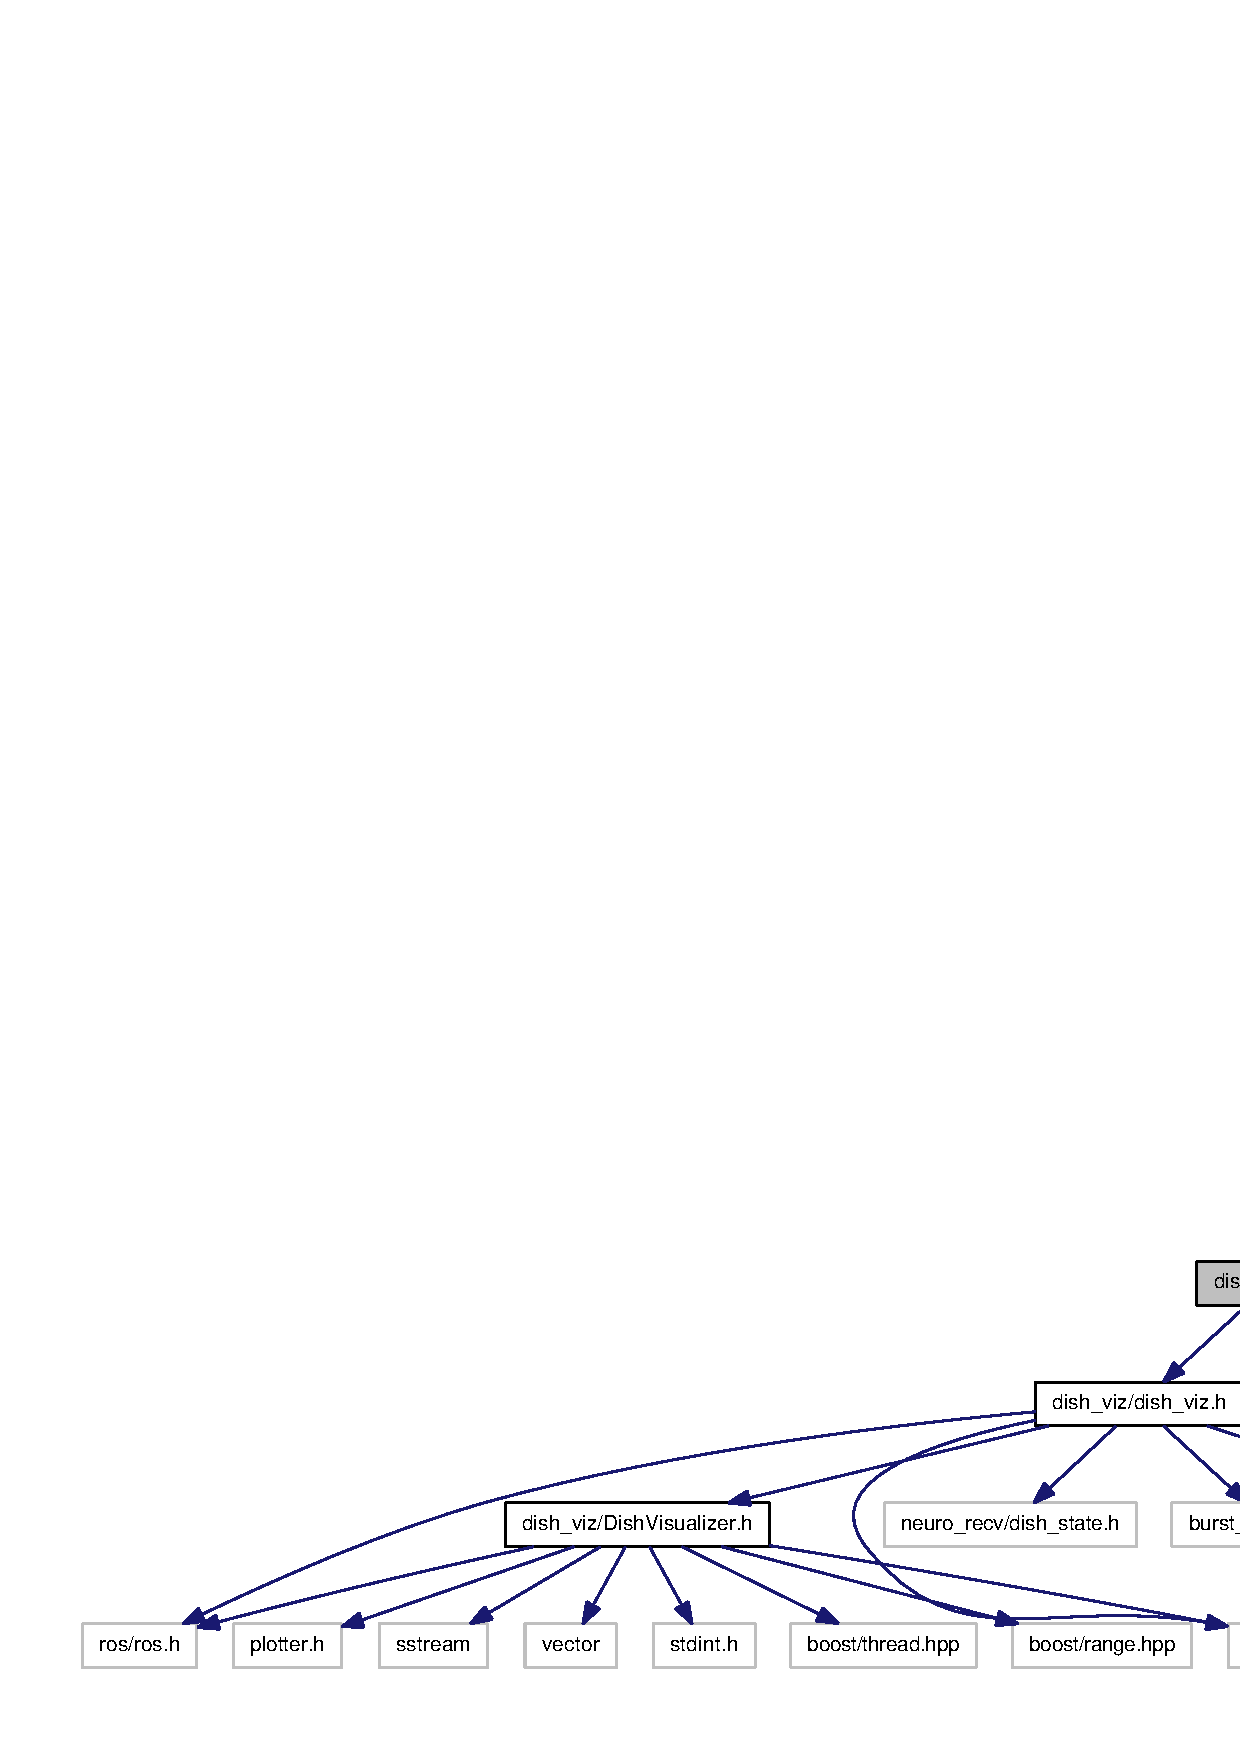
\includegraphics[width=350pt]{dish__viz_8cpp__incl}
\end{center}
\end{figure}
\subsection*{\-Functions}
\begin{DoxyCompactItemize}
\item 
int {\bf main} (int argc, char $\ast$$\ast$argv)
\begin{DoxyCompactList}\small\item\em \-Creates an instance of the node. \end{DoxyCompactList}\end{DoxyCompactItemize}


\subsection{\-Function \-Documentation}
\index{dish\-\_\-viz.\-cpp@{dish\-\_\-viz.\-cpp}!main@{main}}
\index{main@{main}!dish_viz.cpp@{dish\-\_\-viz.\-cpp}}
\subsubsection[{main}]{\setlength{\rightskip}{0pt plus 5cm}int {\bf main} (
\begin{DoxyParamCaption}
\item[{int}]{argc, }
\item[{char $\ast$$\ast$}]{argv}
\end{DoxyParamCaption}
)}\label{dish__viz_8cpp_a3c04138a5bfe5d72780bb7e82a18e627}


\-Creates an instance of the node. 



\-Definition at line 223 of file dish\-\_\-viz.\-cpp.


\section{dish\-\_\-viz.\-h \-File \-Reference}
\label{dish__viz_8h}\index{dish\-\_\-viz.\-h@{dish\-\_\-viz.\-h}}
{\ttfamily \#include \char`\"{}ros/ros.\-h\char`\"{}}\*
{\ttfamily \#include \char`\"{}dish\-\_\-viz/\-Dish\-Visualizer.\-h\char`\"{}}\*
{\ttfamily \#include \char`\"{}neuro\-\_\-recv/dish\-\_\-state.\-h\char`\"{}}\*
{\ttfamily \#include \char`\"{}burst\-\_\-calc/ca.\-h\char`\"{}}\*
{\ttfamily \#include \char`\"{}burst\-\_\-calc/burst.\-h\char`\"{}}\*
{\ttfamily \#include \char`\"{}burst\-\_\-calc/ranges.\-h\char`\"{}}\*
{\ttfamily \#include $<$queue$>$}\*
{\ttfamily \#include $<$string$>$}\*
\-Include dependency graph for dish\-\_\-viz.\-h\-:\nopagebreak
\begin{figure}[H]
\begin{center}
\leavevmode
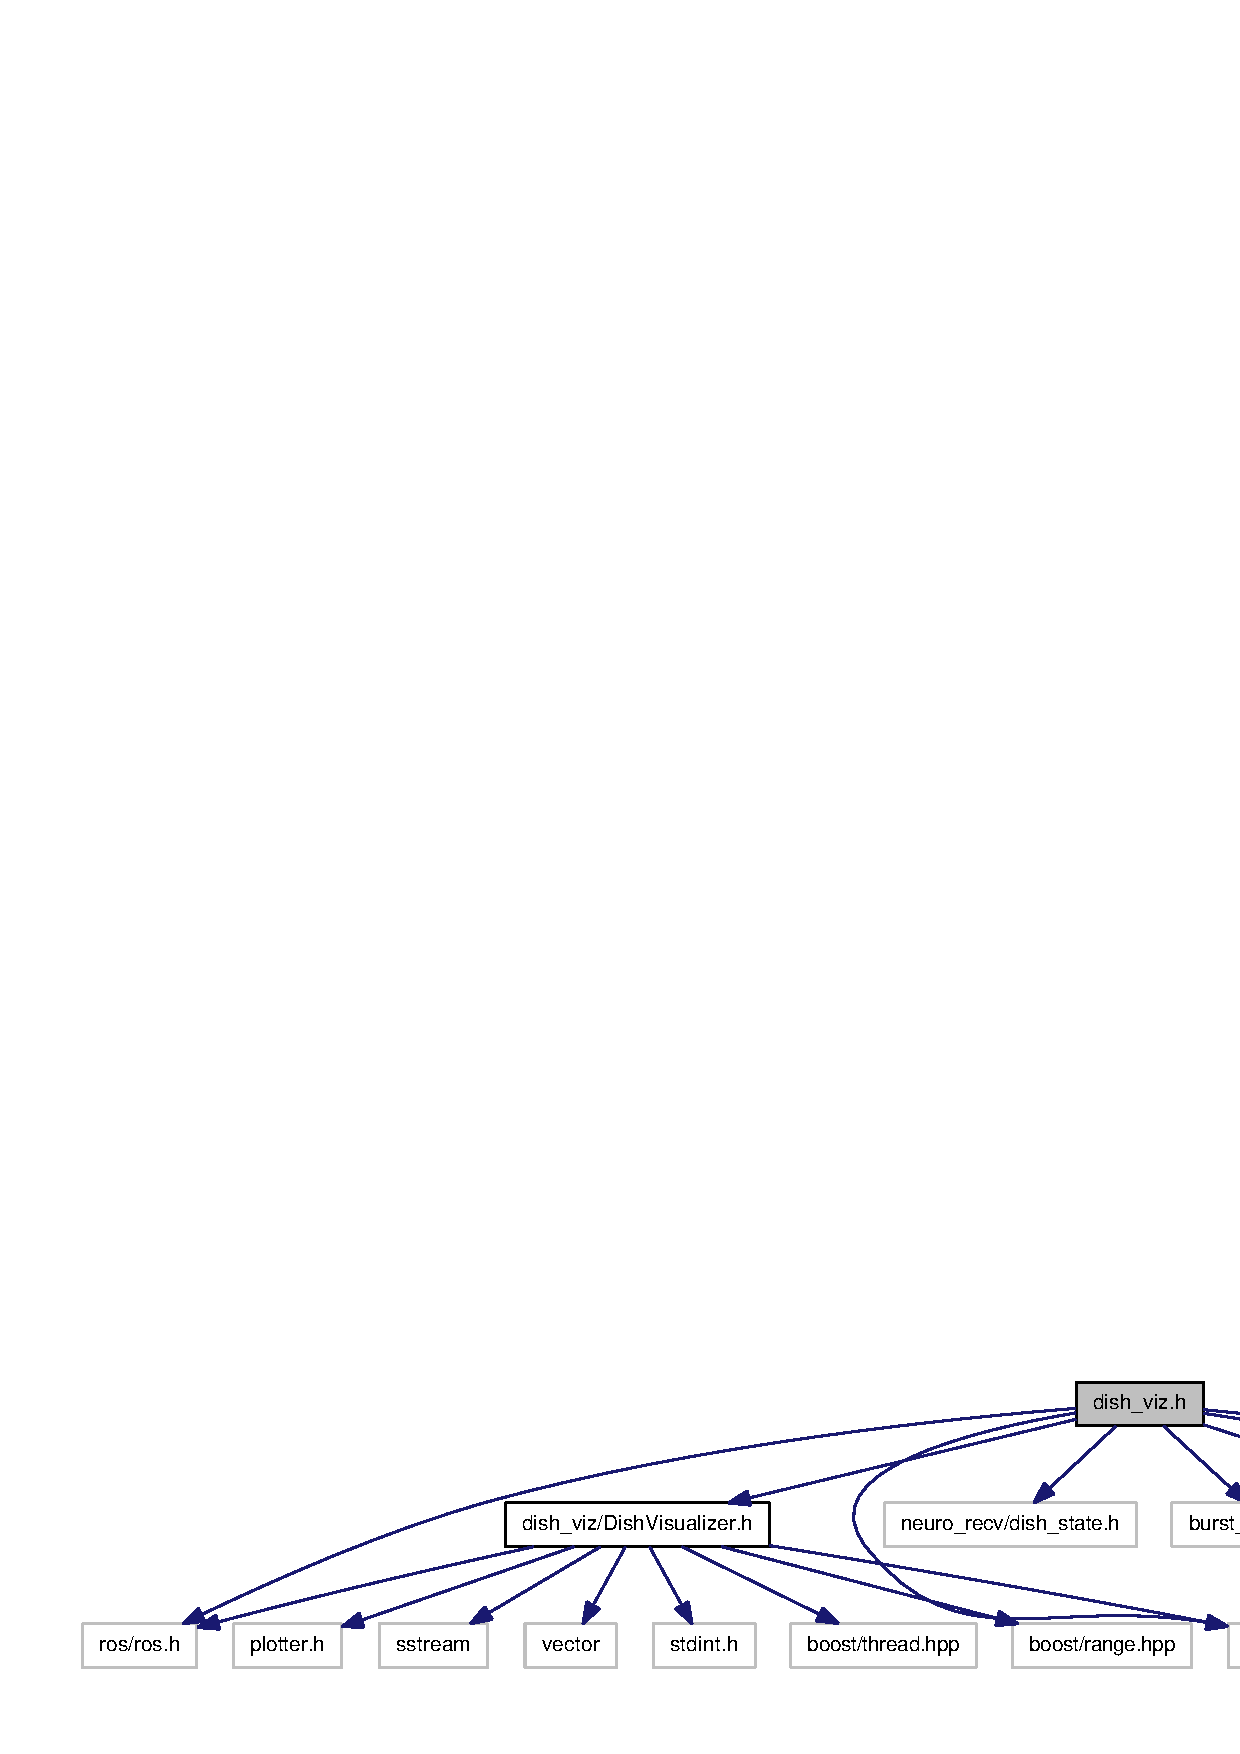
\includegraphics[width=350pt]{dish__viz_8h__incl}
\end{center}
\end{figure}
\-This graph shows which files directly or indirectly include this file\-:\nopagebreak
\begin{figure}[H]
\begin{center}
\leavevmode
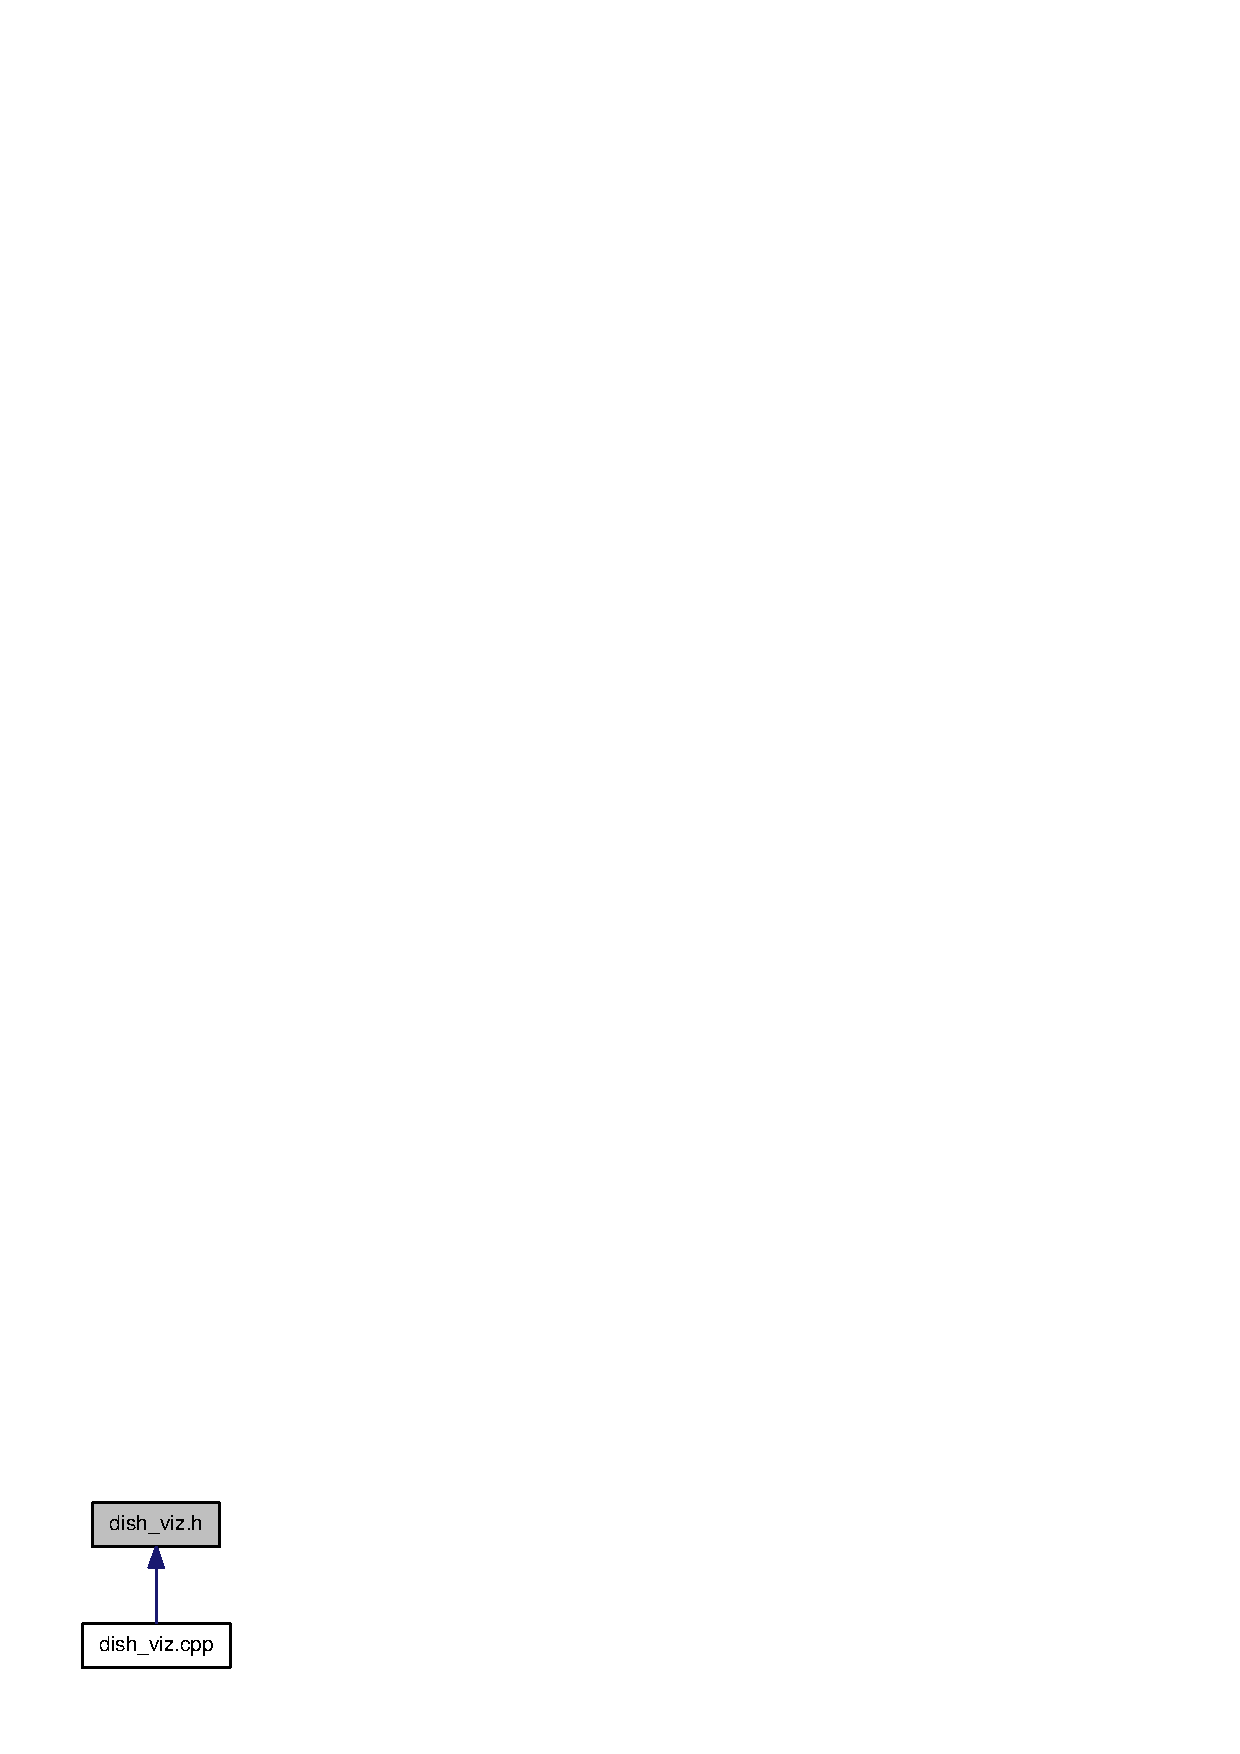
\includegraphics[width=114pt]{dish__viz_8h__dep__incl}
\end{center}
\end{figure}
\subsection*{\-Classes}
\begin{DoxyCompactItemize}
\item 
class {\bf \-Data\-Handler}
\begin{DoxyCompactList}\small\item\em \-Node for visualing dish activity. \end{DoxyCompactList}\end{DoxyCompactItemize}

\section{\-Dish\-Visualizer.\-cpp \-File \-Reference}
\label{DishVisualizer_8cpp}\index{\-Dish\-Visualizer.\-cpp@{\-Dish\-Visualizer.\-cpp}}
{\ttfamily \#include \char`\"{}dish\-\_\-viz/\-Dish\-Visualizer.\-h\char`\"{}}\*
\-Include dependency graph for \-Dish\-Visualizer.\-cpp\-:\nopagebreak
\begin{figure}[H]
\begin{center}
\leavevmode
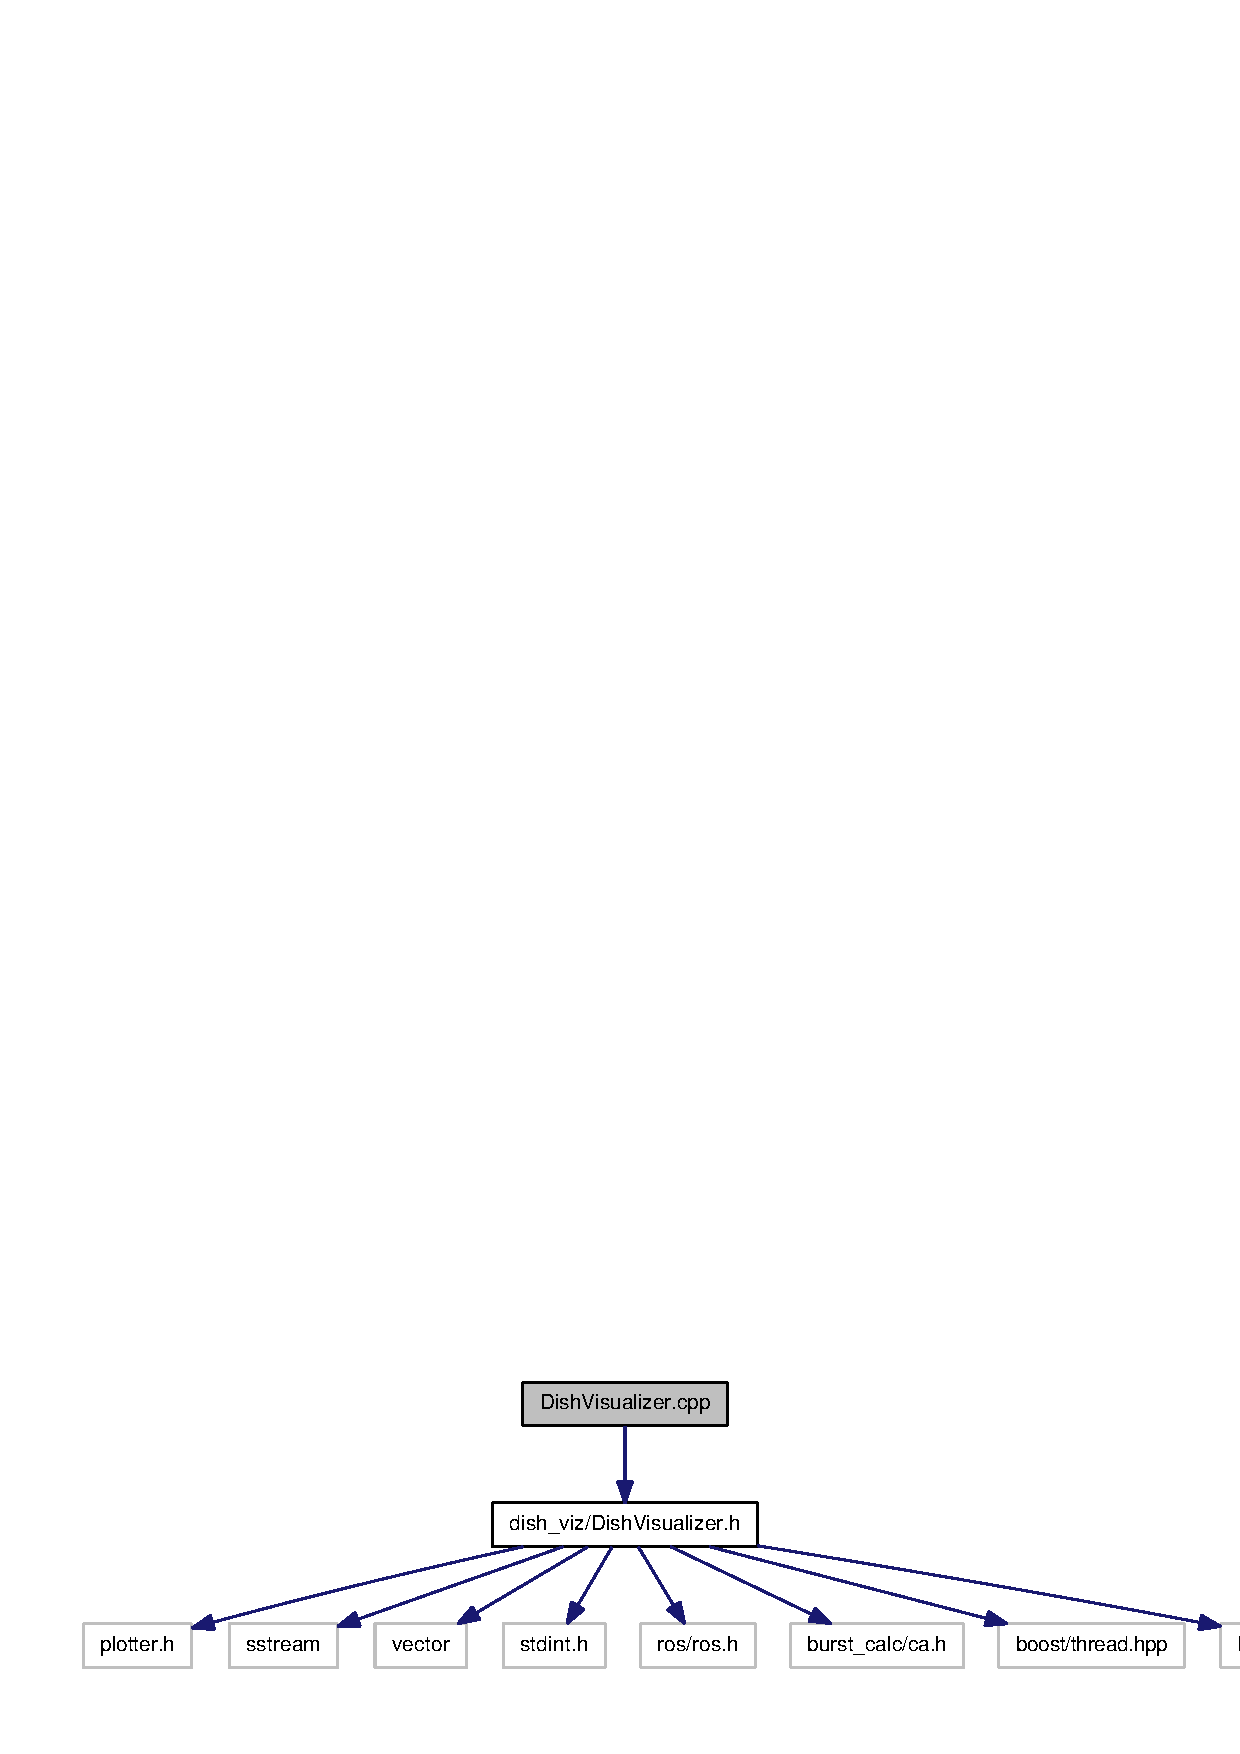
\includegraphics[width=350pt]{DishVisualizer_8cpp__incl}
\end{center}
\end{figure}
\subsection*{\-Defines}
\begin{DoxyCompactItemize}
\item 
\#define {\bf \-C\-O\-L\-S}~{\bf \-R\-O\-W\-S}
\item 
\#define {\bf \-P\-\_\-\-H\-E\-I\-G\-H\-T}~{\bf \-P\-\_\-\-W\-I\-D\-T\-H}
\item 
\#define {\bf \-P\-\_\-\-W\-I\-D\-T\-H}~((7 $\ast$ {\bf \-R\-A\-D\-I\-U\-S}) + (8 $\ast$ (2 $\ast$ {\bf \-R\-A\-D\-I\-U\-S})) + (2 $\ast$ {\bf \-R\-A\-D\-I\-U\-S}))
\item 
\#define {\bf \-R\-A\-D\-I\-U\-S}~20
\item 
\#define {\bf \-R\-O\-W\-S}~8
\item 
\#define {\bf \-S\-T\-A\-R\-T\-\_\-\-X}~(2$\ast${\bf \-R\-A\-D\-I\-U\-S})
\item 
\#define {\bf \-S\-T\-A\-R\-T\-\_\-\-Y}~{\bf \-S\-T\-A\-R\-T\-\_\-\-X}
\item 
\#define {\bf \-X\-\_\-\-S\-T\-E\-P}~(3$\ast${\bf \-R\-A\-D\-I\-U\-S})
\item 
\#define {\bf \-Y\-\_\-\-S\-T\-E\-P}~{\bf \-X\-\_\-\-S\-T\-E\-P}
\end{DoxyCompactItemize}


\subsection{\-Define \-Documentation}
\index{\-Dish\-Visualizer.\-cpp@{\-Dish\-Visualizer.\-cpp}!\-C\-O\-L\-S@{\-C\-O\-L\-S}}
\index{\-C\-O\-L\-S@{\-C\-O\-L\-S}!DishVisualizer.cpp@{\-Dish\-Visualizer.\-cpp}}
\subsubsection[{\-C\-O\-L\-S}]{\setlength{\rightskip}{0pt plus 5cm}\#define {\bf \-C\-O\-L\-S}~{\bf \-R\-O\-W\-S}}\label{DishVisualizer_8cpp_ab59ad2ee1a48b83c2eef1f019ed8cc48}


\-Definition at line 17 of file \-Dish\-Visualizer.\-cpp.

\index{\-Dish\-Visualizer.\-cpp@{\-Dish\-Visualizer.\-cpp}!\-P\-\_\-\-H\-E\-I\-G\-H\-T@{\-P\-\_\-\-H\-E\-I\-G\-H\-T}}
\index{\-P\-\_\-\-H\-E\-I\-G\-H\-T@{\-P\-\_\-\-H\-E\-I\-G\-H\-T}!DishVisualizer.cpp@{\-Dish\-Visualizer.\-cpp}}
\subsubsection[{\-P\-\_\-\-H\-E\-I\-G\-H\-T}]{\setlength{\rightskip}{0pt plus 5cm}\#define {\bf \-P\-\_\-\-H\-E\-I\-G\-H\-T}~{\bf \-P\-\_\-\-W\-I\-D\-T\-H}}\label{DishVisualizer_8cpp_a583315bc971adced4da9397b50384f8f}


\-Definition at line 11 of file \-Dish\-Visualizer.\-cpp.

\index{\-Dish\-Visualizer.\-cpp@{\-Dish\-Visualizer.\-cpp}!\-P\-\_\-\-W\-I\-D\-T\-H@{\-P\-\_\-\-W\-I\-D\-T\-H}}
\index{\-P\-\_\-\-W\-I\-D\-T\-H@{\-P\-\_\-\-W\-I\-D\-T\-H}!DishVisualizer.cpp@{\-Dish\-Visualizer.\-cpp}}
\subsubsection[{\-P\-\_\-\-W\-I\-D\-T\-H}]{\setlength{\rightskip}{0pt plus 5cm}\#define {\bf \-P\-\_\-\-W\-I\-D\-T\-H}~((7 $\ast$ {\bf \-R\-A\-D\-I\-U\-S}) + (8 $\ast$ (2 $\ast$ {\bf \-R\-A\-D\-I\-U\-S})) + (2 $\ast$ {\bf \-R\-A\-D\-I\-U\-S}))}\label{DishVisualizer_8cpp_a351b091c08a4d51a2712f07173ee3b9f}


\-Definition at line 10 of file \-Dish\-Visualizer.\-cpp.

\index{\-Dish\-Visualizer.\-cpp@{\-Dish\-Visualizer.\-cpp}!\-R\-A\-D\-I\-U\-S@{\-R\-A\-D\-I\-U\-S}}
\index{\-R\-A\-D\-I\-U\-S@{\-R\-A\-D\-I\-U\-S}!DishVisualizer.cpp@{\-Dish\-Visualizer.\-cpp}}
\subsubsection[{\-R\-A\-D\-I\-U\-S}]{\setlength{\rightskip}{0pt plus 5cm}\#define {\bf \-R\-A\-D\-I\-U\-S}~20}\label{DishVisualizer_8cpp_aa4f8ea40228c3c3a9a7143b1d1ad8956}


\-Definition at line 9 of file \-Dish\-Visualizer.\-cpp.

\index{\-Dish\-Visualizer.\-cpp@{\-Dish\-Visualizer.\-cpp}!\-R\-O\-W\-S@{\-R\-O\-W\-S}}
\index{\-R\-O\-W\-S@{\-R\-O\-W\-S}!DishVisualizer.cpp@{\-Dish\-Visualizer.\-cpp}}
\subsubsection[{\-R\-O\-W\-S}]{\setlength{\rightskip}{0pt plus 5cm}\#define {\bf \-R\-O\-W\-S}~8}\label{DishVisualizer_8cpp_a3cfd3aa62338d12609f6d65bce97e9cd}


\-Definition at line 16 of file \-Dish\-Visualizer.\-cpp.

\index{\-Dish\-Visualizer.\-cpp@{\-Dish\-Visualizer.\-cpp}!\-S\-T\-A\-R\-T\-\_\-\-X@{\-S\-T\-A\-R\-T\-\_\-\-X}}
\index{\-S\-T\-A\-R\-T\-\_\-\-X@{\-S\-T\-A\-R\-T\-\_\-\-X}!DishVisualizer.cpp@{\-Dish\-Visualizer.\-cpp}}
\subsubsection[{\-S\-T\-A\-R\-T\-\_\-\-X}]{\setlength{\rightskip}{0pt plus 5cm}\#define {\bf \-S\-T\-A\-R\-T\-\_\-\-X}~(2$\ast${\bf \-R\-A\-D\-I\-U\-S})}\label{DishVisualizer_8cpp_aa7f8bac4ff85ad501e926167631749bb}


\-Definition at line 14 of file \-Dish\-Visualizer.\-cpp.

\index{\-Dish\-Visualizer.\-cpp@{\-Dish\-Visualizer.\-cpp}!\-S\-T\-A\-R\-T\-\_\-\-Y@{\-S\-T\-A\-R\-T\-\_\-\-Y}}
\index{\-S\-T\-A\-R\-T\-\_\-\-Y@{\-S\-T\-A\-R\-T\-\_\-\-Y}!DishVisualizer.cpp@{\-Dish\-Visualizer.\-cpp}}
\subsubsection[{\-S\-T\-A\-R\-T\-\_\-\-Y}]{\setlength{\rightskip}{0pt plus 5cm}\#define {\bf \-S\-T\-A\-R\-T\-\_\-\-Y}~{\bf \-S\-T\-A\-R\-T\-\_\-\-X}}\label{DishVisualizer_8cpp_ae28b1a95ee25def272409b9b8ce57f73}


\-Definition at line 15 of file \-Dish\-Visualizer.\-cpp.

\index{\-Dish\-Visualizer.\-cpp@{\-Dish\-Visualizer.\-cpp}!\-X\-\_\-\-S\-T\-E\-P@{\-X\-\_\-\-S\-T\-E\-P}}
\index{\-X\-\_\-\-S\-T\-E\-P@{\-X\-\_\-\-S\-T\-E\-P}!DishVisualizer.cpp@{\-Dish\-Visualizer.\-cpp}}
\subsubsection[{\-X\-\_\-\-S\-T\-E\-P}]{\setlength{\rightskip}{0pt plus 5cm}\#define {\bf \-X\-\_\-\-S\-T\-E\-P}~(3$\ast${\bf \-R\-A\-D\-I\-U\-S})}\label{DishVisualizer_8cpp_adcf8217a358479af0f61f56de1c8e396}


\-Definition at line 12 of file \-Dish\-Visualizer.\-cpp.

\index{\-Dish\-Visualizer.\-cpp@{\-Dish\-Visualizer.\-cpp}!\-Y\-\_\-\-S\-T\-E\-P@{\-Y\-\_\-\-S\-T\-E\-P}}
\index{\-Y\-\_\-\-S\-T\-E\-P@{\-Y\-\_\-\-S\-T\-E\-P}!DishVisualizer.cpp@{\-Dish\-Visualizer.\-cpp}}
\subsubsection[{\-Y\-\_\-\-S\-T\-E\-P}]{\setlength{\rightskip}{0pt plus 5cm}\#define {\bf \-Y\-\_\-\-S\-T\-E\-P}~{\bf \-X\-\_\-\-S\-T\-E\-P}}\label{DishVisualizer_8cpp_ae9e31004fb9430917b01ba9236799e4f}


\-Definition at line 13 of file \-Dish\-Visualizer.\-cpp.


\section{\-Dish\-Visualizer.\-h \-File \-Reference}
\label{DishVisualizer_8h}\index{\-Dish\-Visualizer.\-h@{\-Dish\-Visualizer.\-h}}
{\ttfamily \#include $<$plotter.\-h$>$}\*
{\ttfamily \#include $<$sstream$>$}\*
{\ttfamily \#include $<$vector$>$}\*
{\ttfamily \#include $<$stdint.\-h$>$}\*
{\ttfamily \#include \char`\"{}ros/ros.\-h\char`\"{}}\*
{\ttfamily \#include \char`\"{}burst\-\_\-calc/ca.\-h\char`\"{}}\*
{\ttfamily \#include \char`\"{}boost/thread.\-hpp\char`\"{}}\*
{\ttfamily \#include \char`\"{}boost/range.\-hpp\char`\"{}}\*
\-Include dependency graph for \-Dish\-Visualizer.\-h\-:\nopagebreak
\begin{figure}[H]
\begin{center}
\leavevmode
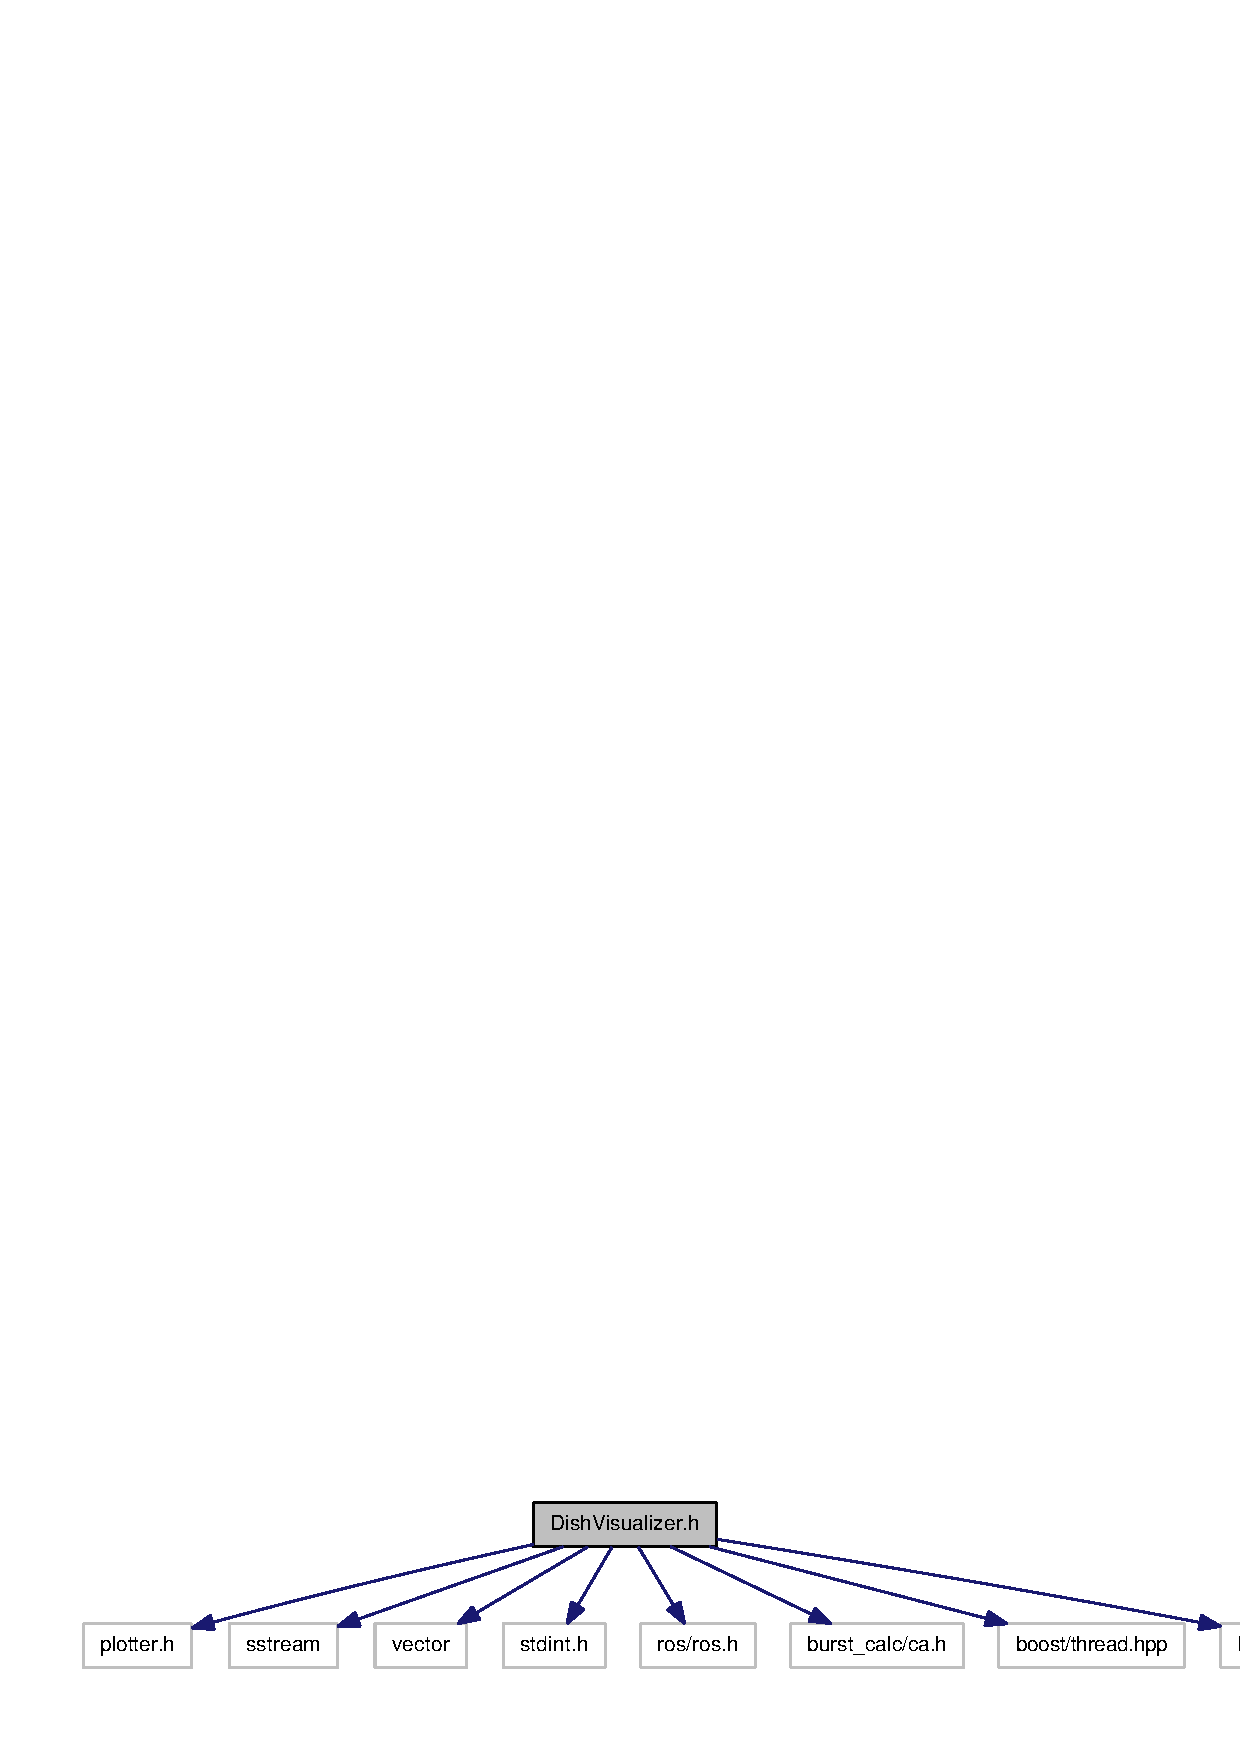
\includegraphics[width=350pt]{DishVisualizer_8h__incl}
\end{center}
\end{figure}
\-This graph shows which files directly or indirectly include this file\-:\nopagebreak
\begin{figure}[H]
\begin{center}
\leavevmode
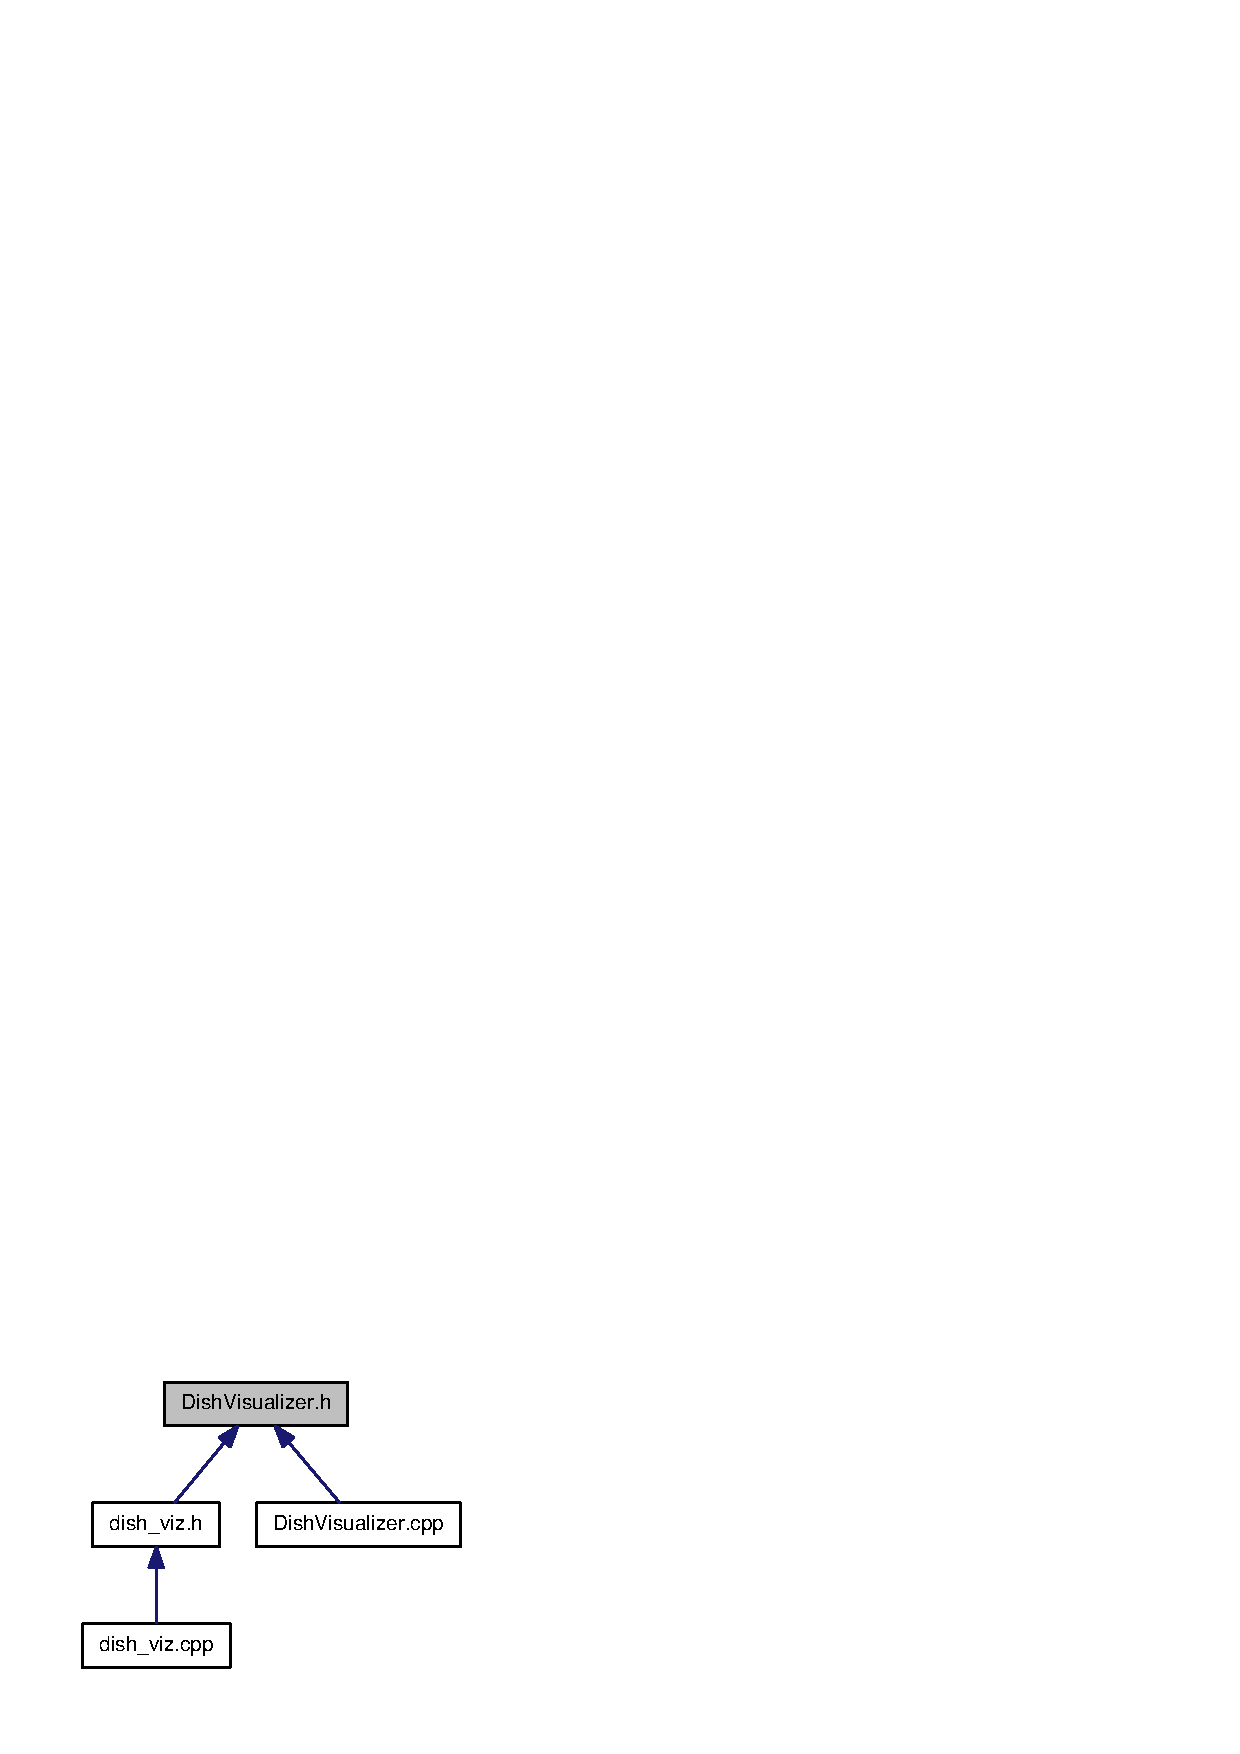
\includegraphics[width=225pt]{DishVisualizer_8h__dep__incl}
\end{center}
\end{figure}
\subsection*{\-Classes}
\begin{DoxyCompactItemize}
\item 
class {\bf \-Dish\-Visualizer}
\begin{DoxyCompactList}\small\item\em \-Helper class for the \doxyref{dish\-\_\-viz}{p.}{namespacedish__viz} node. \end{DoxyCompactList}\end{DoxyCompactItemize}
\subsection*{\-Defines}
\begin{DoxyCompactItemize}
\item 
\#define {\bf \-B\-L\-U\-E\-\_\-\-O\-N\-L\-Y}~3
\item 
\#define {\bf \-M\-A\-X\-\_\-\-C\-O\-L\-O\-R}~65535
\item 
\#define {\bf \-R\-E\-D\-\_\-\-B\-L\-U\-E\-\_\-\-M\-I\-X}~1
\item 
\#define {\bf \-R\-E\-D\-\_\-\-B\-L\-U\-E\-\_\-\-S\-E\-P\-A\-R\-A\-T\-E\-D}~0
\item 
\#define {\bf \-R\-E\-D\-\_\-\-G\-R\-E\-E\-N\-\_\-\-B\-L\-U\-E}~2
\end{DoxyCompactItemize}


\subsection{\-Define \-Documentation}
\index{\-Dish\-Visualizer.\-h@{\-Dish\-Visualizer.\-h}!\-B\-L\-U\-E\-\_\-\-O\-N\-L\-Y@{\-B\-L\-U\-E\-\_\-\-O\-N\-L\-Y}}
\index{\-B\-L\-U\-E\-\_\-\-O\-N\-L\-Y@{\-B\-L\-U\-E\-\_\-\-O\-N\-L\-Y}!DishVisualizer.h@{\-Dish\-Visualizer.\-h}}
\subsubsection[{\-B\-L\-U\-E\-\_\-\-O\-N\-L\-Y}]{\setlength{\rightskip}{0pt plus 5cm}\#define {\bf \-B\-L\-U\-E\-\_\-\-O\-N\-L\-Y}~3}\label{DishVisualizer_8h_a4fb9eab85646daff2a2d45f7cde5b13c}


\-Definition at line 22 of file \-Dish\-Visualizer.\-h.

\index{\-Dish\-Visualizer.\-h@{\-Dish\-Visualizer.\-h}!\-M\-A\-X\-\_\-\-C\-O\-L\-O\-R@{\-M\-A\-X\-\_\-\-C\-O\-L\-O\-R}}
\index{\-M\-A\-X\-\_\-\-C\-O\-L\-O\-R@{\-M\-A\-X\-\_\-\-C\-O\-L\-O\-R}!DishVisualizer.h@{\-Dish\-Visualizer.\-h}}
\subsubsection[{\-M\-A\-X\-\_\-\-C\-O\-L\-O\-R}]{\setlength{\rightskip}{0pt plus 5cm}\#define {\bf \-M\-A\-X\-\_\-\-C\-O\-L\-O\-R}~65535}\label{DishVisualizer_8h_a06e884cefba9e5c96e18ba7e0891a896}


\-Definition at line 24 of file \-Dish\-Visualizer.\-h.

\index{\-Dish\-Visualizer.\-h@{\-Dish\-Visualizer.\-h}!\-R\-E\-D\-\_\-\-B\-L\-U\-E\-\_\-\-M\-I\-X@{\-R\-E\-D\-\_\-\-B\-L\-U\-E\-\_\-\-M\-I\-X}}
\index{\-R\-E\-D\-\_\-\-B\-L\-U\-E\-\_\-\-M\-I\-X@{\-R\-E\-D\-\_\-\-B\-L\-U\-E\-\_\-\-M\-I\-X}!DishVisualizer.h@{\-Dish\-Visualizer.\-h}}
\subsubsection[{\-R\-E\-D\-\_\-\-B\-L\-U\-E\-\_\-\-M\-I\-X}]{\setlength{\rightskip}{0pt plus 5cm}\#define {\bf \-R\-E\-D\-\_\-\-B\-L\-U\-E\-\_\-\-M\-I\-X}~1}\label{DishVisualizer_8h_a2c7f2832037963f9db44f04cdec0fe71}


\-Definition at line 20 of file \-Dish\-Visualizer.\-h.

\index{\-Dish\-Visualizer.\-h@{\-Dish\-Visualizer.\-h}!\-R\-E\-D\-\_\-\-B\-L\-U\-E\-\_\-\-S\-E\-P\-A\-R\-A\-T\-E\-D@{\-R\-E\-D\-\_\-\-B\-L\-U\-E\-\_\-\-S\-E\-P\-A\-R\-A\-T\-E\-D}}
\index{\-R\-E\-D\-\_\-\-B\-L\-U\-E\-\_\-\-S\-E\-P\-A\-R\-A\-T\-E\-D@{\-R\-E\-D\-\_\-\-B\-L\-U\-E\-\_\-\-S\-E\-P\-A\-R\-A\-T\-E\-D}!DishVisualizer.h@{\-Dish\-Visualizer.\-h}}
\subsubsection[{\-R\-E\-D\-\_\-\-B\-L\-U\-E\-\_\-\-S\-E\-P\-A\-R\-A\-T\-E\-D}]{\setlength{\rightskip}{0pt plus 5cm}\#define {\bf \-R\-E\-D\-\_\-\-B\-L\-U\-E\-\_\-\-S\-E\-P\-A\-R\-A\-T\-E\-D}~0}\label{DishVisualizer_8h_aca7b516377ce964b3425a69d32c75b48}


\-Definition at line 19 of file \-Dish\-Visualizer.\-h.

\index{\-Dish\-Visualizer.\-h@{\-Dish\-Visualizer.\-h}!\-R\-E\-D\-\_\-\-G\-R\-E\-E\-N\-\_\-\-B\-L\-U\-E@{\-R\-E\-D\-\_\-\-G\-R\-E\-E\-N\-\_\-\-B\-L\-U\-E}}
\index{\-R\-E\-D\-\_\-\-G\-R\-E\-E\-N\-\_\-\-B\-L\-U\-E@{\-R\-E\-D\-\_\-\-G\-R\-E\-E\-N\-\_\-\-B\-L\-U\-E}!DishVisualizer.h@{\-Dish\-Visualizer.\-h}}
\subsubsection[{\-R\-E\-D\-\_\-\-G\-R\-E\-E\-N\-\_\-\-B\-L\-U\-E}]{\setlength{\rightskip}{0pt plus 5cm}\#define {\bf \-R\-E\-D\-\_\-\-G\-R\-E\-E\-N\-\_\-\-B\-L\-U\-E}~2}\label{DishVisualizer_8h_a818535a0f76c71cfebdb455df86b29c9}


\-Definition at line 21 of file \-Dish\-Visualizer.\-h.


\section{mainpage.\-dox \-File \-Reference}
\label{mainpage_8dox}\index{mainpage.\-dox@{mainpage.\-dox}}

\printindex
\end{document}
